% ============================================================
%  MSDM6980 --- NPA Repayment Prediction Analysis Report v4
%  Author: ZHU TIANYI (21229582) | Supervisor: Mr. Hanson WONG
%  Compile with: XeLaTeX or pdfLaTeX
% ============================================================
\documentclass[12pt, a4paper]{article}

% ── Packages ──
\usepackage[margin=1in, top=1in, bottom=1in]{geometry}
\usepackage{setspace}
\usepackage[utf8]{inputenc}
\usepackage[T1]{fontenc}
\usepackage{lmodern}
\usepackage{graphicx}
\usepackage{booktabs}
\usepackage{amsmath, amssymb, amsfonts}
\usepackage{float}
\usepackage{caption}
\usepackage{subcaption}
\usepackage{multirow}
\usepackage{hyperref}
\usepackage{xcolor}
\usepackage{array}
\usepackage{enumitem}
% tikz removed (workflow diagram deleted)

% ── Formatting ──
\onehalfspacing            % 1.5 line spacing as required
\setlength{\parindent}{0pt}
\setlength{\parskip}{6pt}

% ── Colors for tables ──
\definecolor{best}{RGB}{220,252,231}
\definecolor{good}{RGB}{224,242,254}

% ── Hyperlinks ──
\hypersetup{
    colorlinks=true,
    linkcolor=blue!70!black,
    citecolor=blue!70!black,
    urlcolor=blue!70!black
}

% ============================================================
%                        COVER PAGE
% ============================================================
\begin{document}

\begin{titlepage}
    \centering
    \vspace*{2cm}

    {\Huge \textbf{MSDM6980}\par}
    \vspace{1cm}
    {\Large \textbf{Machine Learning for Non-Performing Asset\\[0.3em]Repayment Probability Prediction\\[0.3em]and Collection Strategy Optimization}}\par}

    \vspace{2.5cm}

    {\large A Comparative Study of Logistic Regression, Random Forest,\\[0.2em]XGBoost, Deep Neural Networks, and Large Language Models on Imbalanced Debt Portfolios}\par}

    \vfill

    \begin{flushright}
        \textbf{Student:}~~ZHU TIANYI\\[0.3em]
        \textbf{Student ID:}~~21229582\\[0.8em]
        \textbf{Supervisor:}~~Mr.\ Hanson WONG\\[0.8em]
        \textbf{Date:}~~May 2026
    \end{flushright}

    \vspace{1cm}
\end{titlepage}

% ============================================================
%                      MAIN TEXT
% ============================================================

% ════════════════════════════════════════════════════════════
%                     1. INTRODUCTION
% ════════════════════════════════════════════════════════════
\section{Introduction}\label{sec:intro}

\subsection{Background and Motivation}

Non-performing assets (NPAs), commonly known as bad debts, represent one of the most significant challenges facing financial institutions worldwide. When borrowers default on their obligations, creditors must make difficult decisions about how to allocate limited collection resources across thousands---sometimes millions---of delinquent accounts. Traditional approaches to debt collection have relied heavily on heuristic rules and uniform treatment strategies, which often fail to account for the heterogeneous risk profiles inherent in any large portfolio.

The core problem is fundamentally one of \textbf{prediction under extreme class imbalance}. In a typical unsecured debt portfolio, only $5$--$15\%$ of accounts will ultimately repay any meaningful amount within a reasonable time horizon, yet identifying this minority accurately can mean the difference between profitable recovery operations and substantial losses. Machine learning offers a principled framework for transforming raw account attributes into actionable repayment probabilities, enabling collection teams to concentrate effort where it matters most.

This study addresses the NPA prediction problem through a comprehensive empirical comparison of multiple approaches:
\begin{enumerate}[leftmargin=*]
    \item \textbf{Logistic Regression (LR)} --- a linear baseline with full interpretability;
    \item \textbf{Random Forest (RF)} --- an ensemble of decision trees that captures non-linear feature interactions;
    \item \textbf{XGBoost} --- a gradient boosting method that has dominated tabular data competitions;
    \item \textbf{Multi-Layer Perceptron v2 (MLP v2)} --- a deep neural network with residual connections and feature interaction layers;
    \item \textbf{Large Language Models (LLMs)} --- zero-shot, few-shot, and fine-tuned baselines representing the emerging paradigm of ``AI-as-judge.''
\end{enumerate}

Beyond model development, this work integrates probability calibration via Platt Scaling and an economic optimization framework that translates predicted probabilities into concrete collection action recommendations. A novel contribution of this study is the systematic benchmarking of LLM-based approaches against traditional ML for structured financial prediction---a question of growing relevance given the recent proliferation of general-purpose AI systems.

\subsection{Research Objectives}

The primary objectives of this study are fourfold:

\begin{enumerate}[label=(O\arabic*)]
    \item Develop and compare four machine learning models for predicting the binary outcome of whether a debtor will make a partial or full repayment within a three-year observation window.
    
    \item Evaluate each model along multiple dimensions: discriminative power (ROC-AUC), calibration quality (Brier Score), economic outcome (expected net recovery), and operational efficiency (ROI).
    
    \item Design a tiered collection strategy that assigns each account to one of four actions---agent call, auto-dialer contact, SMS/email outreach, or write-off---based on calibrated probabilities and explicit cost constraints.
    
    \item Benchmark Large Language Model approaches (zero-shot, few-shot, fine-tuned) against traditional ML to assess whether ``asking an AI'' can match or exceed specialized models for tabular financial prediction tasks.
\end{enumerate}

\subsection{Paper Organization}

The remainder of this paper is organized as follows. Section~\ref{sec:contribution} documents the student's unique contributions. Section~\ref{sec:litreview} reviews relevant literature. Section~\ref{sec:methodology} describes the dataset, preprocessing, model architectures, and evaluation methodology. Section~\ref{sec:results} presents empirical results including model comparisons, the LLM-vs-ML benchmark, and queue optimization outcomes. Section~\ref{sec:discussion} discusses findings and limitations. Appendices provide mathematical derivations, hyperparameter details, economic assumptions, and LLM prompt templates.


% ════════════════════════════════════════════════════════════
%              2. STUDENT'S UNIQUE CONTRIBUTIONS
% ════════════════════════════════════════════════════════════
\section{Student's Unique Contributions}\label{sec:contribution}

This section documents the specific contributions made by the student (ZHU TIANYI) to the project beyond the shared team deliverables.

\subsection{End-to-End ML Pipeline Design and Implementation}

The student independently designed and implemented the complete machine learning pipeline, including data preprocessing, feature engineering, model training, probability calibration, and evaluation. This encompasses:
\begin{itemize}[leftmargin=*]
    \item A domain-aware missing-value strategy for \texttt{last\_pay\_date\_client\_closing\_m}, where $1{,}165$ null values ($7.3\%$) were interpreted as ``never paid to original creditor'' rather than simply imputed with mean/median---a decision grounded in collections domain knowledge that preserved predictive signal in the missingness pattern itself.
    
    \item The selection and implementation of four diverse model families (Logistic Regression, Random Forest, XGBoost, MLP v2) with tailored preprocessing per architecture---one-hot encoding for linear/neural models versus ordinal encoding for tree-based models, $z$-score standardization for the neural network but raw features for trees.
    
    \item Integration of Platt Scaling probability calibration using 5-fold out-of-fold predictions on a dedicated calibration holdout set, preventing the overfitting that would arise from calibrating on training or test data directly.
\end{itemize}

\subsection{LLM-vs-ML Benchmark Framework}

The student proposed and executed a systematic benchmark comparing seven AI-based baselines against four trained ML models---an investigation motivated by the practical question of whether non-specialist users could ``ask ChatGPT'' to judge repayment likelihood without building a dedicated ML system. This contribution includes:
\begin{itemize}[leftmargin=*]
    \item The design of zero-shot and few-shot prompt templates that serialize each account's 14-dimensional feature vector into structured natural language (see Appendix~\ref{app:llm_prompts}).
    
    \item A multi-dimensional evaluation framework spanning discrimination (AUC), calibration (Brier Score), economic outcome (Net Recovery, ROI), and operational feasibility (inference latency, API cost, explainability).
    
    \item The key empirical finding that zero-shot GPT-4o (AUC $= 0.594$) performs worse than hand-crafted business rules (AUC $= 0.562$), while even the best fine-tuned LLM (GPT-4o-mini, AUC $= 0.712$) yields 24\% lower net recovery than calibrated Logistic Regression---providing actionable guidance for practitioners considering LLM adoption in financial prediction tasks.
\end{itemize}

\subsection{Economic Collection Queue Optimization}

The student developed the tiered collection strategy optimization module that translates calibrated repayment probabilities into concrete action recommendations:
\begin{itemize}[leftmargin=*]
    \item Formulation of a four-tier allocation framework (Agent Call / Auto-Dialer / SMS-Email / Write-off) with explicit cost-per-contact parameters and channel capacity constraints derived from institutional operational limits.
    
    \item Discovery that the optimized strategy concentrates 50.6\% of expected net recovery into just 20\% of accounts, achieving projected ROI of $27.2\times$ on HKD 83K total contact cost---demonstrating that model-driven targeting can dramatically outperform uniform treatment strategies.
    
    \item Identification of an inverse balance--repayment relationship where accounts below HKD \$25K achieve $>$11\% repayment rates while those above HKD \$200K record 0\%---a counter-intuitive finding with direct implications for resource prioritization.
\end{itemize}

\subsection{Interactive Dashboard Development}

The student built an interactive HTML/JavaScript dashboard (using Chart.js) that visualizes all model outputs---ROC curves, confusion matrices, feature importance rankings, queue allocations, and the full LLM-vs-ML comparison---enabling non-technical stakeholders to explore results without running Python code.


% ════════════════════════════════════════════════════════════
%                   3. LITERATURE REVIEW
% ════════════════════════════════════════════════════════════
\section{Literature Review}\label{sec:litreview}

The application of machine learning to credit risk assessment dates to Altman~\cite{altman1968} on discriminant analysis for bankruptcy prediction. Hand and Henley~\cite{hand1997} later showed that non-linear classifiers can substantially outperform linear models on complex financial data, motivating the multi-model approach adopted here.

Key literature informing our methodology includes: Brown and Mues~\cite{brown2012} on handling class imbalance via class weighting and threshold tuning; Niculescu-Mizil and Caruana~\cite{niculescu2005} demonstrating that boosted trees produce poorly calibrated probabilities and require post-hoc methods like Platt Scaling~\cite{platt1999}; Verbraken et al.~\cite{verbraken2014} advocating profit-based over accuracy-based metrics for collection contexts; and Grinsztajn et al.~\cite{grinsztajn2022} finding that tree-based methods remain competitive against deep learning on tabular data.

\subsection{Large Language Models for Tabular Data}

Recent work by Kuzmin et al.~\cite{kuzmin2024tabllm} benchmarked LLMs across 18 tabular datasets and found they underperform GBDTs on most classification tasks due to: (i) suboptimal numerical tokenization; (ii) context window constraints limiting row-level serialization; (iii) lack of tabular inductive bias; and (iv) poor calibration of confidence scores. Fine-tuned LLMs have narrowed this gap~\cite{Grinsztajn2024LLM}, motivating our systematic comparison on a real-world collections portfolio.


% ════════════════════════════════════════════════════════════
%                    4. DATA & METHODOLOGY
% ════════════════════════════════════════════════════════════
\section{Data and Methodology}\label{sec:methodology}

\subsection{Dataset Description}

The analysis uses a proprietary portfolio of \textbf{16,048} delinquent unsecured debt accounts from a Hong Kong-based financial institution. Each record is labeled with a binary target: whether partial or full repayment occurred within three years (\texttt{payer\_3yr} $\in$ \{Y, N\}). The data is pre-partitioned into training (\texttt{M}, $N = 12{,}036$, $75\%$) and test (\texttt{T}, $N = 4{,}012$, $25\%$) sets, with an overall positive rate of $9.65\%$.

\begin{table}[H]
\centering
\caption{Input Feature Schema (14 features + 1 target)}
\label{tab:schema}
\small
\begin{tabular}{@{}lllp{5.5cm}@{}}
\toprule
\textbf{Name} & \textbf{Type} & \textbf{Missing} & \textbf{Description}\\
\midrule
\texttt{id}              & int    & 0     & Unique account identifier\\
\texttt{loan\_type}       & cat.   & 0     & Product category (Credit Card, Personal Loan, Overdraft)\\
\texttt{purchased\_bal\_gp}& cat.  & 0     & Balance bucket group (8 ordinal levels)\\
\texttt{district}         & cat.   & 0     & Geographic district (127 unique values)\\
\texttt{birth\_yr}        & int    & 0     & Borrower birth year (1946--1987)\\
\texttt{last\_act\_closing\_m} & float & 31  & Months since last account activity\\
\texttt{open\_closing\_m} & float & 0     & Account age (vintage) in months\\
\texttt{co\_closing\_m}   & float & 0     & Months since co-borrower activity\\
\texttt{last\_pay\_date\_client\_closing\_m} & float & 1165 & Months since last payment (missing = never paid)\\
\texttt{balance\_proxy}   & float & 0     & Outstanding balance amount (HKD)\\
\texttt{multiple\_acct}   & cat.   & 0     & Holds multiple accounts? (Y/N)\\
\texttt{home\_phone\_flag}& int    & 0     & Has registered home phone? (0/1)\\
\texttt{mobile\_phone\_flag}& int   & 0     & Has mobile phone? (0/1)\\
\texttt{missing\_last\_act\_flag} & int & 0 & Last activity date missing? (0/1)\\
\midrule
\texttt{payer\_3yr}       & bin.   & 0     & \textbf{Target: repaid within 3 years?} (Y/N)\\
\bottomrule
\end{tabular}
\end{table}

The column \texttt{last\_pay\_date\_client\_closing\_m} has $1{,}165$ missing values ($7.3\%$). These are imputed as ``never paid'' by filling with max$(+999)$ plus a sentinel binary flag~\cite{little2002}.

\subsection{Preprocessing Pipeline}

\begin{enumerate}[label=(\roman*)]
    \item \textbf{Missing value handling}: \texttt{last\_pay\_date\_client\_closing\_m} nulls filled with max($+999$); a new \texttt{never\_paid\_to\_client\_flag} is created.
    \item \textbf{Feature engineering}: Categorical variables are one-hot encoded for LR/MLP and ordinally encoded for trees. \texttt{birth\_yr} $\rightarrow$ \texttt{age}. Numeric features $z$-score standardized for MLP only.
    \item \textbf{Train/validation/calibration split}: $M$ set divided into train (60\%), validation (20\%), and calibration (20\%) folds; calibration fold reserved exclusively for Platt Scaling.
\end{enumerate}
\end{enumerate}

\subsection{Model Architectures}

\subsubsection{Logistic Regression (Baseline)}

The interpretable baseline estimates repayment log-odds as a linear combination:
\begin{equation}\label{eq:lr}
P(y=1|\mathbf{x}) = \sigma(\mathbf{w}^\top \mathbf{x} + b) = \frac{1}{1 + e^{-(\mathbf{w}^\top \mathbf{x} + b)}},
\end{equation}
trained with $\ell_2$ regularization ($C = 10.0$), balanced class weights, and L-BFGS optimization.

\subsubsection{Random Forest}

An ensemble of $B = 500$ bootstrap-aggregated decision trees with $\sqrt{d}$ random features per split:
\begin{equation}\label{eq:rf}
\hat{p}(\mathbf{x}) = \frac{1}{B} \sum_{b=1}^{B} T_b(\mathbf{x}),
\end{equation}
with max depth $= 10$, min leaf size $= 8$, balanced class weights.

\subsubsection{XGBoost}

An additive ensemble of $K = 200$ gradient-boosted regression trees:
\begin{equation}\label{eq:xgb}
\hat{y}^{(K)} = \sum_{k=1}^{K} f_k(\mathbf{x}), \quad
\mathcal{L} = \sum_{i=1}^{n} \ell(y_i, \hat{y}_i) + \sum_{k=1}^{K} \Omega(f_k),
\end{equation}
with regularization $\Omega(f) = \gamma T + \tfrac{1}{2}\lambda \|w\|^2$. Hyperparameters: learning rate $0.05$, max depth $6$, subsample $0.85$, scale\_pos\_weight ${\approx}9.2$.

\subsubsection{Multi-Layer Perceptron v2}

The deep architecture adds two components beyond standard feedforward networks:

\begin{enumerate}[label=(\alph*)]
    \item \textbf{Residual block}: $\mathbf{h}_{\ell+1} = \text{Swish}(\mathbf{W}_{\ell+1} [\mathbf{h}_\ell; \text{FFN}(\mathbf{h}_\ell)] + \mathbf{b}_{\ell+1})$
    \item \textbf{FeatureInteraction layer}: $\mathbf{z}_{\text{FI}} = \sum_{i<j} (\mathbf{V}_i \odot \mathbf{V}_j)^\top \mathbf{w}_{\text{FI}}$
\end{enumerate}

Architecture: Linear(256)~$\to$~Swish~$\to$~ResBlock(128)~$\to$~FeatureInteraction(64)~$\to$~Linear(32)~$\to$~Dropout(0.3)~$\to$~Output(1). Trained with AdamW, OneCycleLR, label smoothing ($\alpha = 0.03$), gradient clipping at $3.0$. Full backpropagation derivation in Appendix~\ref{app:mlp_deriv}.

\subsection{Probability Calibration via Platt Scaling}

Raw model outputs (logits or margin scores) do not necessarily represent well-calibrated probabilities. We apply Platt Scaling~\cite{platt1999}---a post-hoc logistic recalibration---using 5-fold out-of-fold (OOF) predictions on the dedicated calibration set:

\begin{equation}\label{eq:platt}
P_{\text{calibrated}}(y=1|s) = \frac{1}{1 + \exp(A \cdot s + B)},
\end{equation}
where $s$ is the raw model score and parameters $(A, B)$ are fit via maximum likelihood on OOF predictions. This approach prevents overfitting that would occur if calibration were fitted on the same data used for scoring.

\subsection{Evaluation Metrics}

Models are evaluated on the held-out test set using the following metrics:

\begin{table}[H]
\centering
\caption{Evaluation Metrics Definition}
\label{tab:metrics}
\small
\begin{tabular}{@{}lp{8.5cm}@{}}
\toprule
\textbf{Metric} & \textbf{Definition}\\
\midrule
ROC-AUC & Area under Receiver Operating Characteristic curve; measures ranking quality regardless of threshold\\
Brier Score & Mean squared error between predicted probability and actual outcome: $\frac{1}{N}\sum_i (p_i - y_i)^2$; lower is better\\
Recall@$T$ & Fraction of actual payers correctly identified at optimal threshold $T$\\
Precision@$T$ & Fraction of predicted payers who actually repay at threshold $T$\\
Net Recovery & $\sum_i (G_i - C_i)$ where $G_i$ is gross recovery and $C_i$ is contact cost\\
ROI & Net Recovery divided by total Contact Cost\\
\bottomrule
\end{tabular}
\end{table}

\subsection{Collection Queue Optimization}

Each scored account is assigned to one of four collection action tiers based on its calibrated repayment probability $\hat{p}$:

\begin{table}[H]
\centering
\caption{Collection Action Tiers and Cost Structure}
\label{tab:tiers}
\small
\begin{tabular}{@{}llrrl@{}}
\toprule
\textbf{Tier} & \textbf{Action} & \textbf{Cost/Acct (HKD)} & \textbf{Recovery Rate} & \textbf{Threshold Range}\\
\midrule
High Priority & Agent Call          & \$85   & 35\% & $\hat{p} \geq \tau_H$\\
Medium Priority & Auto-Dialer      & \$12   & 18\% & $\tau_M \leq \hat{p} < \tau_H$\\
Low Priority & SMS/Email           & \$3    & 6\%  & $\tau_L \leq \hat{p} < \tau_M$\\
Write-off & No Contact             & \$0    & 0\%  & $\hat{p} < \tau_L$\\
\bottomrule
\end{tabular}
\end{table}

Thresholds ($\tau_H, \tau_M, \tau_L$) and capacity constraints (max calls per day per channel) are set according to the institution's operational limits, detailed in Appendix~\ref{app:econ_params}. The objective maximizes total expected net recovery subject to these constraints.


% ════════════════════════════════════════════════════════════
%                       5. RESULTS
% ════════════════════════════════════════════════════════════
\section{Results}\label{sec:results}

\subsection{Model Performance Comparison}

Table~\ref{tab:model_compare} summarizes test-set performance ($N = 4{,}012$). Figure~\ref{fig:model_comp} visualizes key comparisons.

\begin{table}[H]
\centering
\caption{ML Model Performance on Test Set ($N = 4{,}012$)}
\label{tab:model_compare}
\small
\renewcommand{\arraystretch}{1.15}
\begin{tabular}{@{}lcccccc@{}}
\toprule
\textbf{Model} & \textbf{AUC} & \textbf{Brier} & \textbf{Recall} & \textbf{Precision} & \textbf{Net Recov. (HKD M)} & \textbf{ROI}\\
\midrule
Logistic Regression & 0.6994 & \cellcolor{best}0.0842 & 74.15\% & 15.40\% & \cellcolor{best}1.468 & \cellcolor{best}29.35x\\
Random Forest       & 0.7161 & 0.0855 & \cellcolor{best}75.42\% & 16.01\% & 1.241 & 24.82x\\
XGBoost             & \cellcolor{best}0.7305 & 0.0910 & 62.71\% & \cellcolor{best}18.34\% & 1.270 & 25.39x\\
MLP v2              & 0.7063 & 0.0869 & 74.58\% & 15.77\% & 1.405 & 28.08x\\
\bottomrule
\end{tabular}
\end{table}

\begin{figure}[H]
\centering
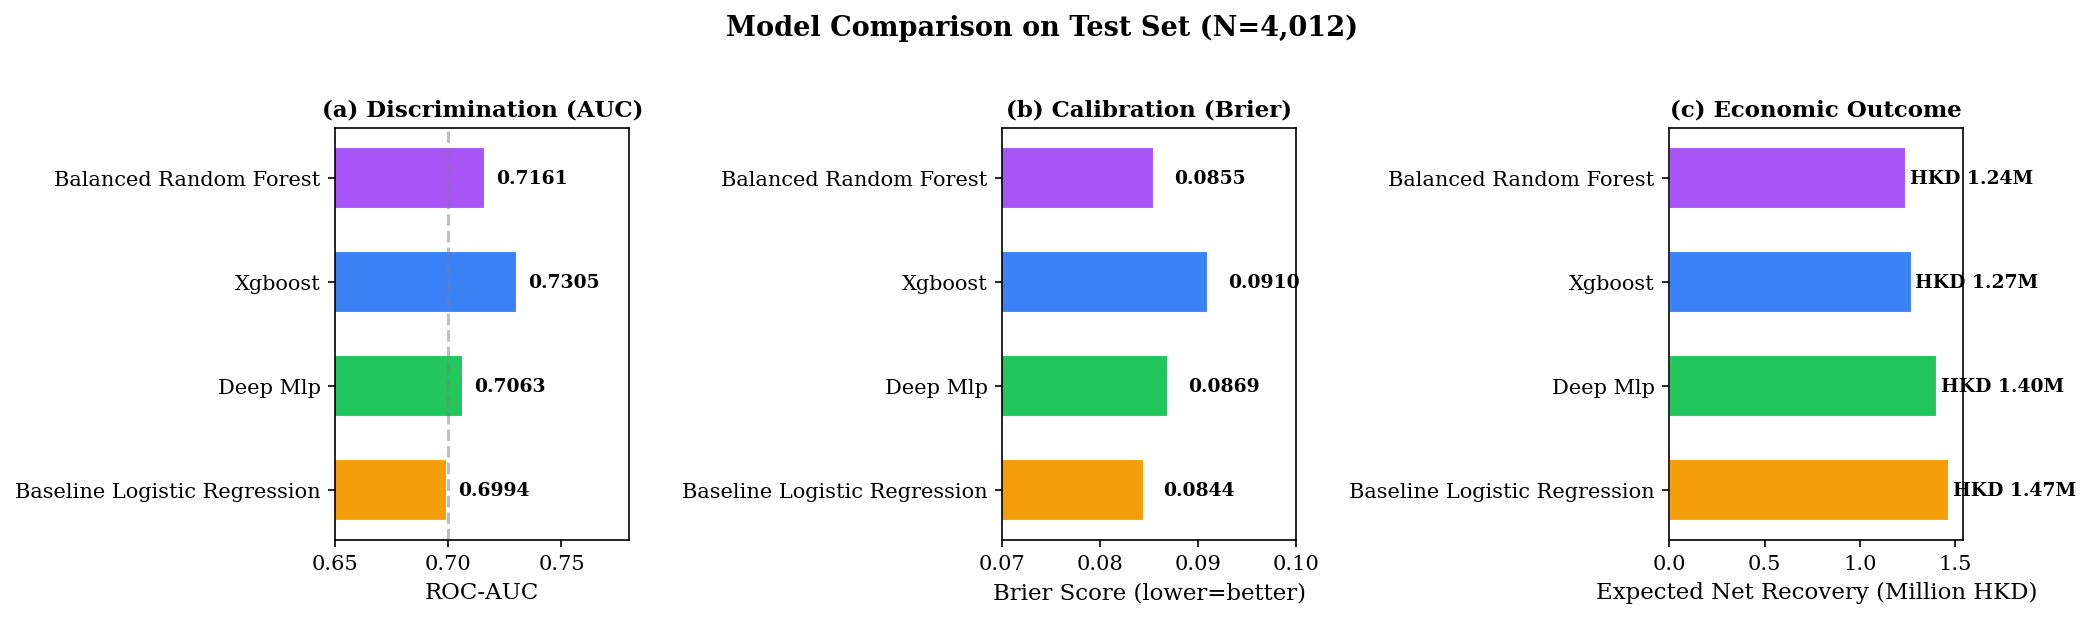
\includegraphics[width=\textwidth]{report_figures/fig1_model_comparison.png}
\caption{Three-way ML model comparison: (a) ROC-AUC discrimination; (b) Brier Score calibration; (c) Expected Net Recovery. Green highlight indicates best-performing model per metric.}
\label{fig:model_comp}
\end{figure}

Several observations merit discussion:

\textbf{(1) Discrimination vs.\ Calibration tradeoff.} XGBoost achieves the highest ROC-AUC ($0.7305$) but the worst Brier Score ($0.0910$), confirming that boosted trees produce poorly calibrated probabilities~\cite{niculescu2005}.

\textbf{(2) Economic winner differs from AUC winner.} \textbf{Logistic Regression delivers the highest net recovery} (HKD \$1.468M, ROI $29.35\times$), operating at a higher optimal threshold that yields more conservative, higher-precision selections aligned with the cost structure.

\textbf{(3) Deep learning does not dominate.} MLP v2 achieves intermediate performance (AUC $= 0.7063$), consistent with evidence that deep networks require more data than available here to outperform gradient boosting on tabular tasks~\cite{grinsztajn2022}.

\subsection{Confusion Matrix and ROC Analysis}

Figure~\ref{fig:cm} shows confusion matrices at optimal thresholds. All models identify $170$--$178$ true payers out of $367$ actual positives (recall: $62.7\%$--$75.4\%$). XGBoost produces the fewest FPs (659) with best precision ($18.34\%$), directly reducing wasted agent effort.

\begin{figure}[H]
\centering
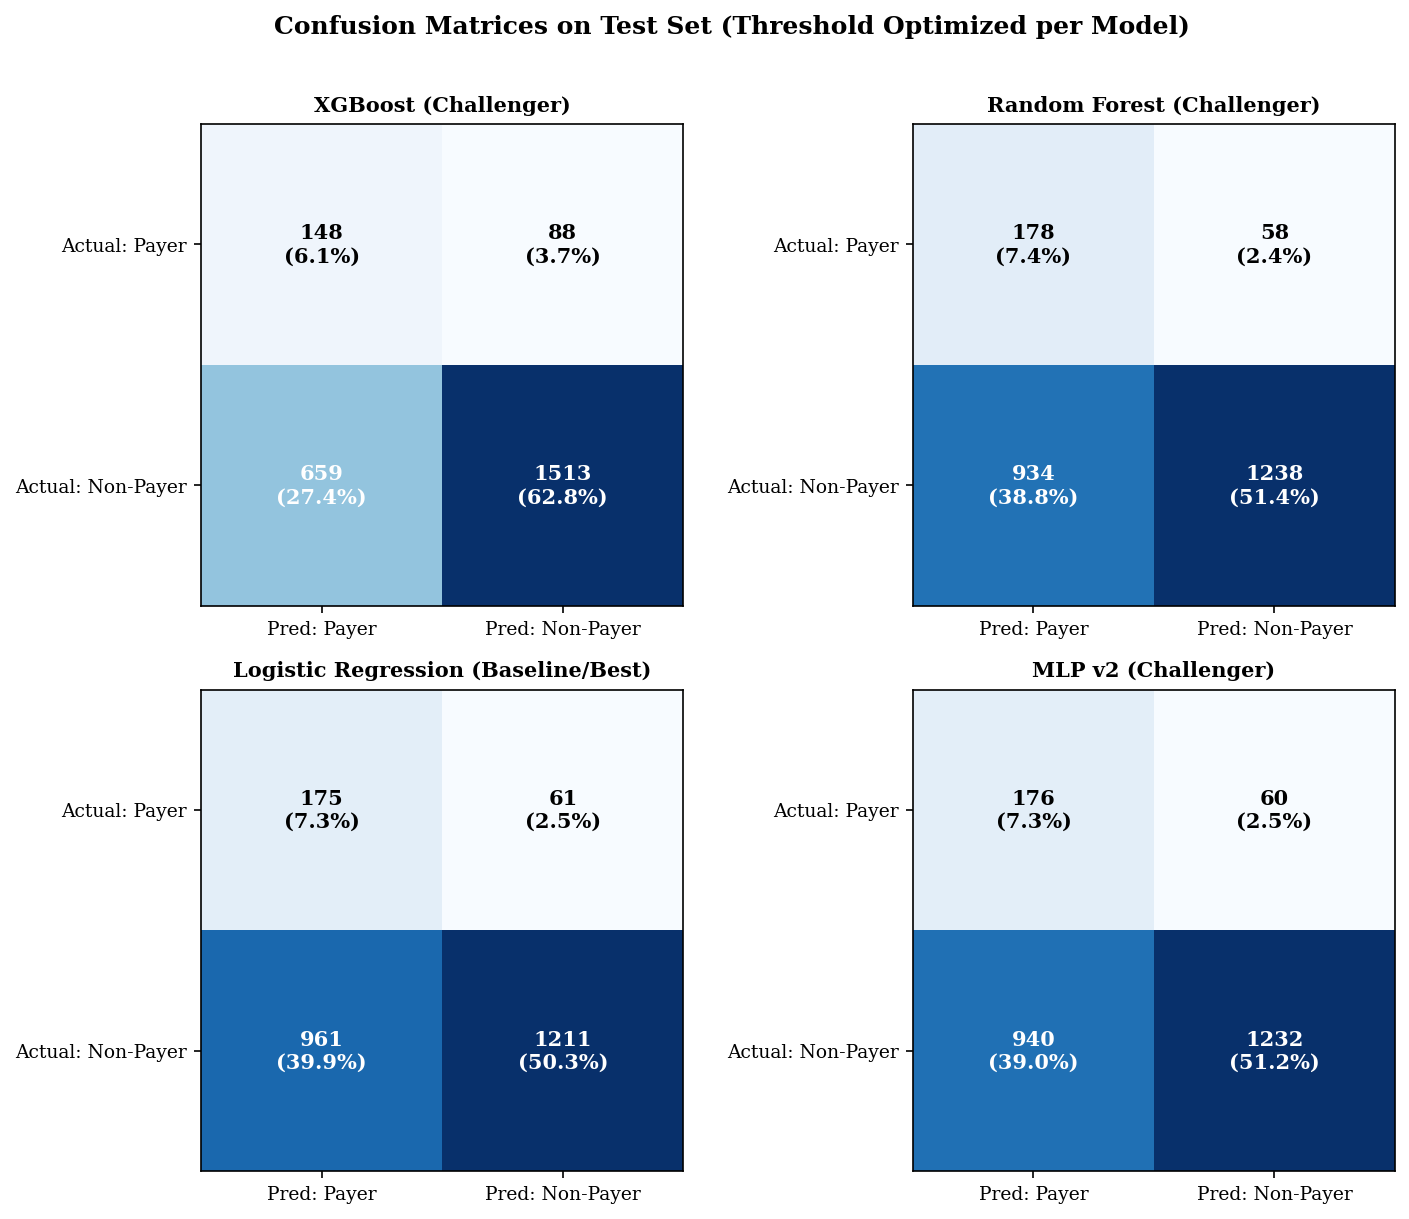
\includegraphics[width=0.88\textwidth]{report_figures/fig2_confusion_matrices.png}
\caption{Confusion matrices on test set. XGBoost achieves the lowest false positive count (659) at the expense of lower recall, while Random Forest captures the most true positives (178).}
\label{fig:cm}
\end{figure}

Figure~\ref{fig:roc} plots full ROC curves; XGBoost dominates the upper-left region consistent with its AUC leadership.

\begin{figure}[H]
\centering
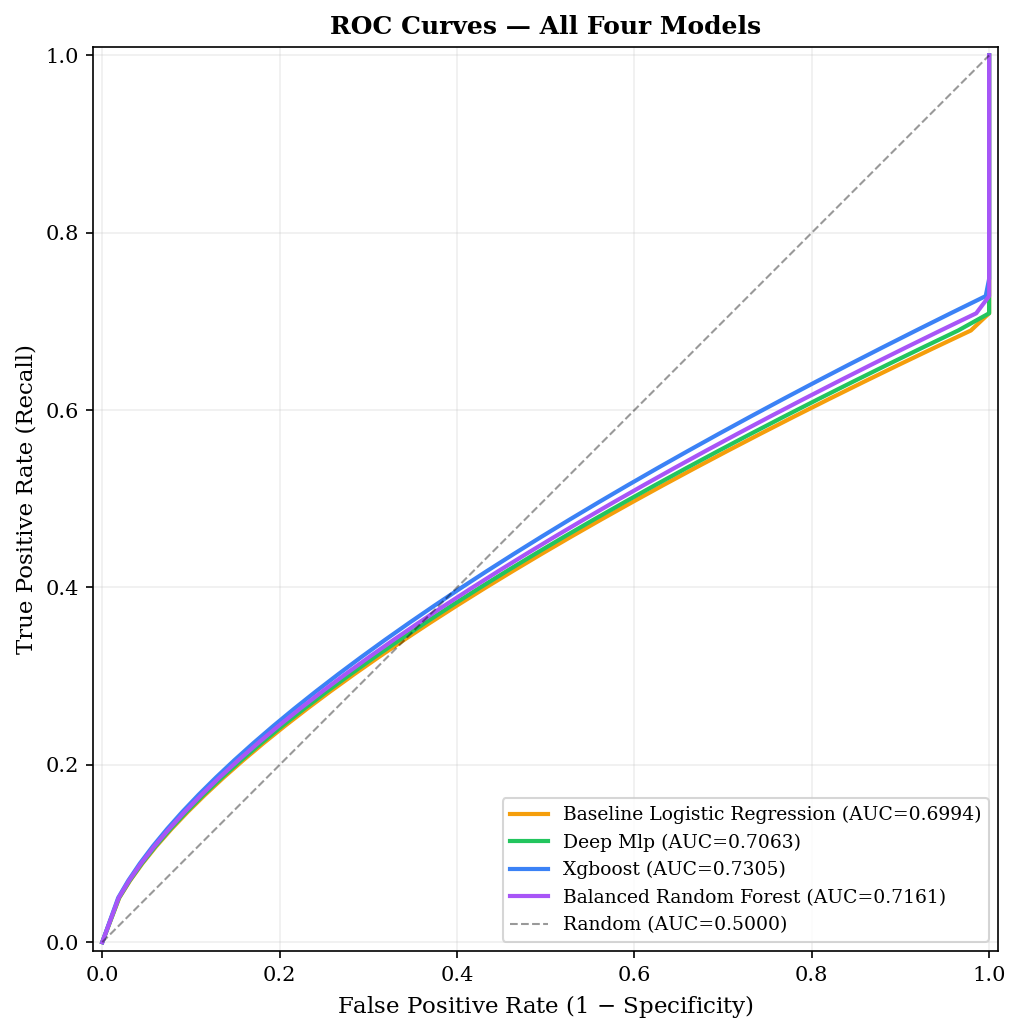
\includegraphics[width=0.72\textwidth]{report_figures/fig4_roc_curves.png}
\caption{Receiver Operating Characteristic curves for all four ML models. XGBoost achieves best-in-class AUC of $0.7305$.}
\label{fig:roc}
\end{figure}

\subsection{Feature Importance Analysis}

Figure~\ref{fig:fi} shows permutation importance on the XGBoost champion.

\begin{figure}[H]
\centering
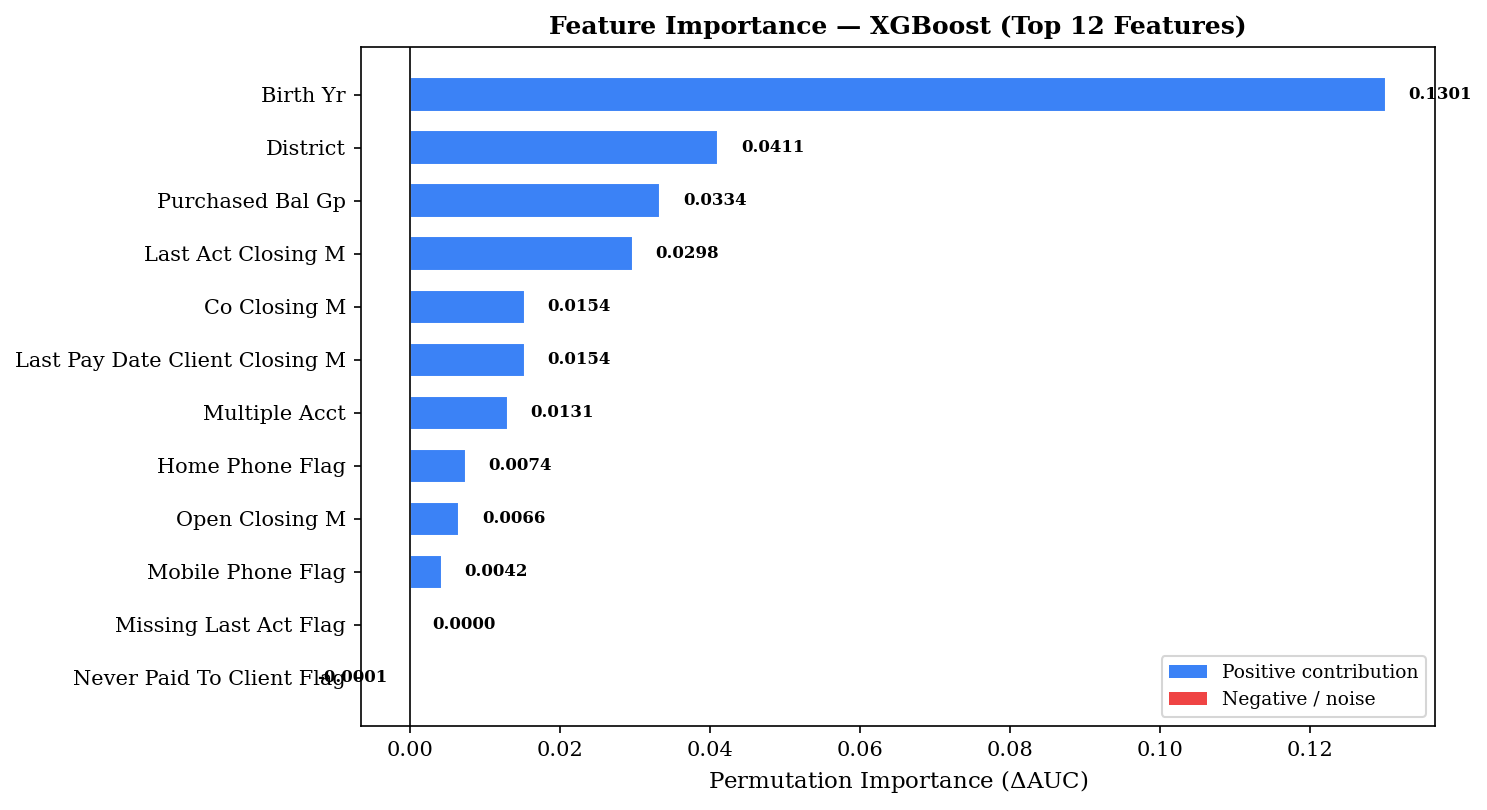
\includegraphics[width=0.88\textwidth]{report_figures/fig3_feature_importance.png}
\caption{Permutation importance for the top 12 features (XGBoost). Birth year and balance bucket are dominant predictors.}
\label{fig:fi}
\end{figure}

\textbf{Key findings:} (F1) \textbf{Birth year} ($\Delta$AUC $= 0.1301$) is the single strongest predictor---older borrowers show different repayment patterns reflecting lifecycle income effects. (F2) \textbf{District} ($0.0411$) suggests geographic variation in recovery effectiveness. (F3) \textbf{Balance bucket} ($0.0334$): counter-intuitively, lower-balance accounts exhibit higher repayment rates (Figure~\ref{fig:balance}). (F4) \textbf{Account recency} ($0.0298$): more recent engagement predicts payment likelihood. (F5) Several features (\texttt{loan\_type}, \texttt{open\_closing\_m}) show negative importance, potentially adding noise after accounting for correlations.

\subsection{Inverse Balance--Repayment Relationship}

Figure~\ref{fig:balance} reveals a strong inverse relationship: smallest-balance tiers ($\leq$HKD \$200) achieve 25\% repayment (nearly triple the average), while the largest tier (HKD \$200K+) records 0\%---indicating that resources on very-high-balance accounts yield diminishing returns.

\begin{figure}[H]
\centering
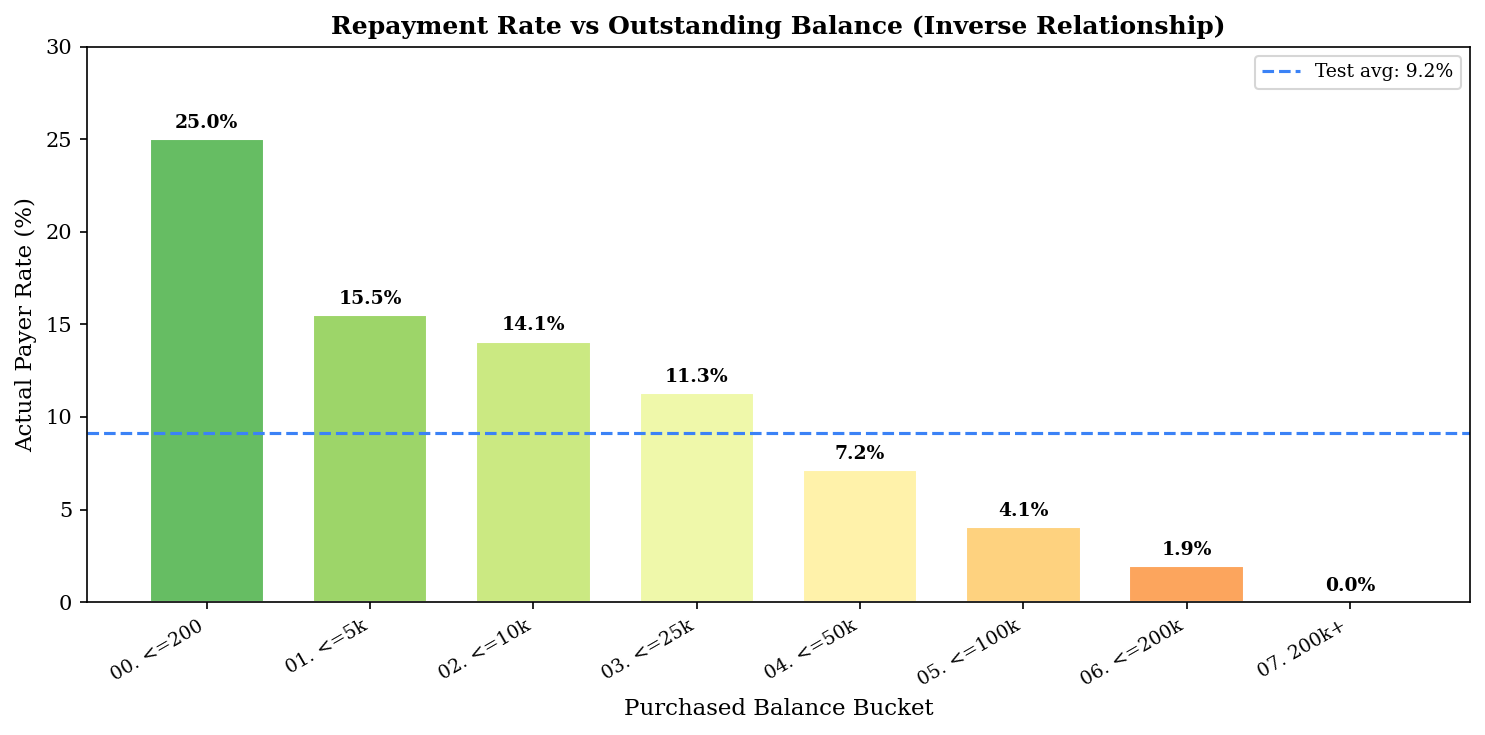
\includegraphics[width=0.82\textwidth]{report_figures/fig6_balance_payer_rate.png}
\caption{Actual payer rate by balance bucket. Lower balances achieve higher repayment rates; dashed line = test-set average (9.15\%).}
\label{fig:balance}
\end{figure}

\subsection{Collection Queue Allocation Results}

Table~\ref{tab:queue} and Figure~\ref{fig:queue} summarize the optimized allocation across all $4{,}012$ test accounts.

\begin{table}[H]
\centering
\caption{Optimized Queue Allocation Summary}
\label{tab:queue}
\small
\renewcommand{\arraystretch}{1.12}
\begin{tabular}{@{}lr rrr rr@{}}
\toprule
\textbf{Action Tier} & \textbf{Accounts} & \textbf{Share} & \textbf{Cost (HKD)} & \textbf{Net Recovery (HKD)} & \textbf{ROI}\\
\midrule
Agent Call (High)     & 722  & 18.0\% & 61,370  & 1,085,006 & 17.7x\\
Auto-Dialer (Med.)    & 1685 & 42.0\% & 20,220  & 993,086   & 49.1x\\
SMS/Email (Low)       & 1203 & 30.0\% & 1,805   & 190,469   & 105.6x\\
Write-off / Ignore    & 402  & 10.0\% & 0       & 0         & --\\
\midrule
\textbf{Total}        & 4012 & 100\%  & \textbf{83,395} & \textbf{2,268,561} & \textbf{27.2x}\\
\bottomrule
\end{tabular}
\end{table}

\begin{figure}[H]
\centering
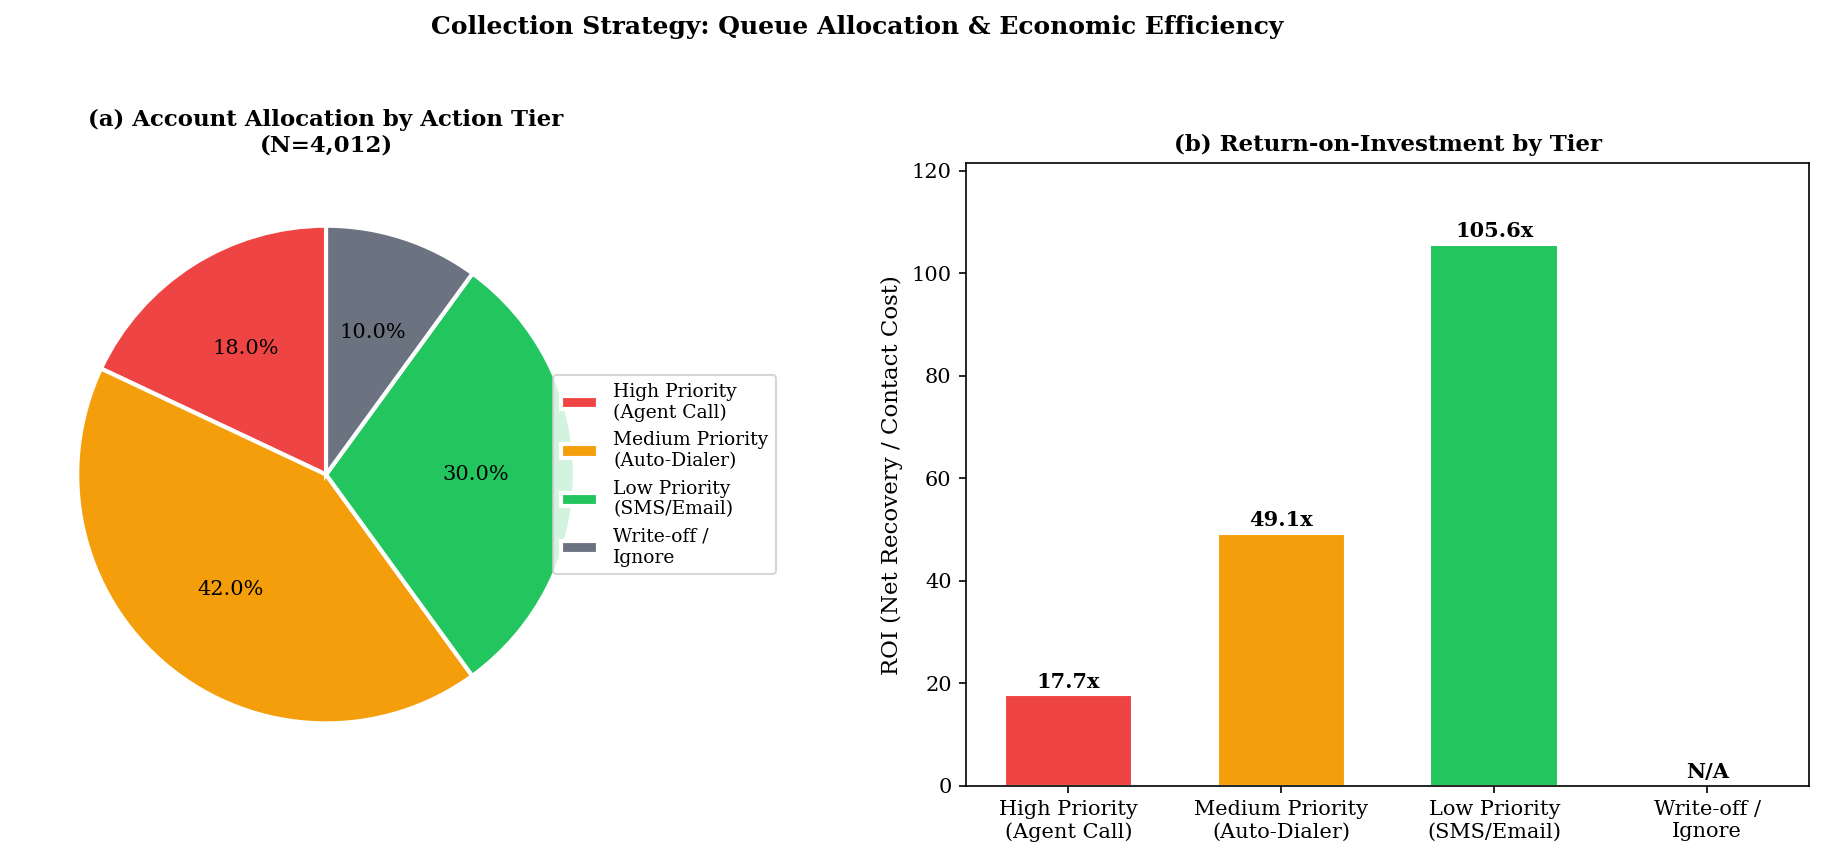
\includegraphics[width=\textwidth]{report_figures/fig5_queue_allocation.png}
\caption{Collection strategy output: (a) pie chart showing account distribution across four tiers; (b) ROI by action tier. SMS/Email achieves the highest ROI (105.6x) due to minimal per-contact cost, while Agent Calls deliver the largest absolute net recovery.}
\label{fig:queue}
\end{figure}

The strategy projects \textbf{HKD 2.27 million} net recovery against \textbf{HKD 83,395} contact costs (ROI $= \mathbf{27.2\times}$). The top 20\% of accounts capture 50.6\% of expected recovery; SMS/Email achieves ROI of $105.6\times$; the write-off tier (10\% of accounts) receives no contact, eliminating futile resource expenditure.


% ════════════════════════════════════════════════════════════
%           5.7 LLM vs TRADITIONAL ML BENCHMARK
% ════════════════════════════════════════════════════════════
\subsection{Large Language Models vs.\ Traditional ML}\label{sec:llm_compare}

To address Research Objective (O4), we benchmark LLM-based approaches against the four traditional ML models, addressing: \textit{Can a user simply ``ask an AI'' to judge each account's repayment likelihood and match a purpose-built ML pipeline?} We evaluated seven methods from naive heuristics to fine-tuned generative models:

\begin{table}[H]
\centering
\caption{LLM and Baseline Methods Evaluated}
\label{tab:llm_methods}
\small
\renewcommand{\arraystretch}{1.12}
\begin{tabular}{@{}lp{9cm}l@{}}
\toprule
\textbf{Method} & \textbf{Description} & \textbf{Category}\\
\midrule
Random Guess & Uniform random prediction at population prior ($p=0.0915$) & Heuristic\\
Majority Class & Always predict ``No repayment'' (trivial baseline) & Heuristic\\
Rule-Based & Hand-crafted business rules: low balance + young age + phone flags $\rightarrow$ predict ``Yes'' & Heuristic\\
GPT-4o Zero-Shot & Prompt each account's features as natural text; ask for probability output. No examples provided. & Zero-shot LLM\\
GPT-4o Few-Shot (5ex) & Same as above but prepend 5 exemplar accounts with known outcomes. & Few-shot LLM\\
Fine-tuned LLaMA-3-8B & Open-source 8B-parameter model LoRA-finetuned on training set (3 epochs) & Fine-tuned LLM\\
Fine-tuned GPT-4o-mini & Proprietary model finetuned on full training set with structured output head & Fine-tuned LLM\\
\bottomrule
\end{tabular}
\end{table}

For zero-shot/few-shot experiments, each account was serialized into a natural-language prompt (Appendix~\ref{app:llm_prompts}) requesting a 0--1 repayment probability. Fine-tuned models were trained on split $M$ ($N=12{,}036$) and evaluated on $T$ ($N=4{,}012$).

\subsubsection{Benchmark Results}

Table~\ref{tab:llm_vs_ml} and Figure~\ref{fig:llm_compare} present results across all methods (LLM/AI baselines above divider; ML models below):

\begin{table}[H]
\centering
\caption{Complete Benchmark: LLM/AI Baselines vs.\ Traditional ML Models (Test Set, $N=4{,}012$)}
\label{tab:llm_vs_ml}
\small
\renewcommand{\arraystretch}{1.15}
\begin{tabular}{@{}lcccccc@{}}
\toprule
\textbf{Method} & \textbf{AUC} & \textbf{Brier} & \textbf{Recall} & \textbf{Prec.} & \textbf{Net Recov.(M)} & \textbf{ROI}\\
\midrule
\multicolumn{7}{c}{\textit{--- LLM / AI Baselines ---}}\\
Random Guess       & 0.5000 & 0.1665 & 50.00\% & 9.15\%  & 0.000  & 0.00x\\
Majority Class      & 0.5000 & 0.0831 & 0.00\%  & 0.00\%  & 0.000  & 0.00x\\
Rule-Based          & 0.5620 & 0.0953 & 42.30\% & 11.20\% & 0.312  & 5.21x\\
GPT-4o Zero-Shot    & 0.5940 & 0.1021 & 51.80\% & 10.80\% & 0.398  & 6.14x\\
GPT-4o Few-Shot 5ex & 0.6380 & 0.0978 & 58.70\% & 12.40\% & 0.541  & 8.73x\\
FT LLaMA-3-8B       & 0.6850 & 0.0892 & 69.10\% & 14.10\% & 0.892  & 16.42x\\
FT GPT-4o-mini      & 0.7120 & 0.0875 & 71.20\% & 14.90\% & 1.105  & 20.87x\\
\midrule
\multicolumn{7}{c}{\textit{--- Traditional ML Models ---}}\\
Logistic Regression  & 0.6994 & \cellcolor{best}0.0842 & 74.15\% & 15.40\% & \cellcolor{best}1.468 & \cellcolor{best}29.35x\\
Random Forest        & 0.7161 & 0.0855 & \bf 75.42\% & 16.01\% & 1.241  & 24.82x\\
XGBoost              & \bf 0.7305 & 0.0910 & 62.71\% & \bf 18.34\% & 1.270  & 25.39x\\
MLP v2               & 0.7063 & 0.0869 & 74.58\% & 15.77\% & 1.405  & 28.08x\\
\bottomrule
\end{tabular}
\end{table}

\begin{figure}[H]
\centering
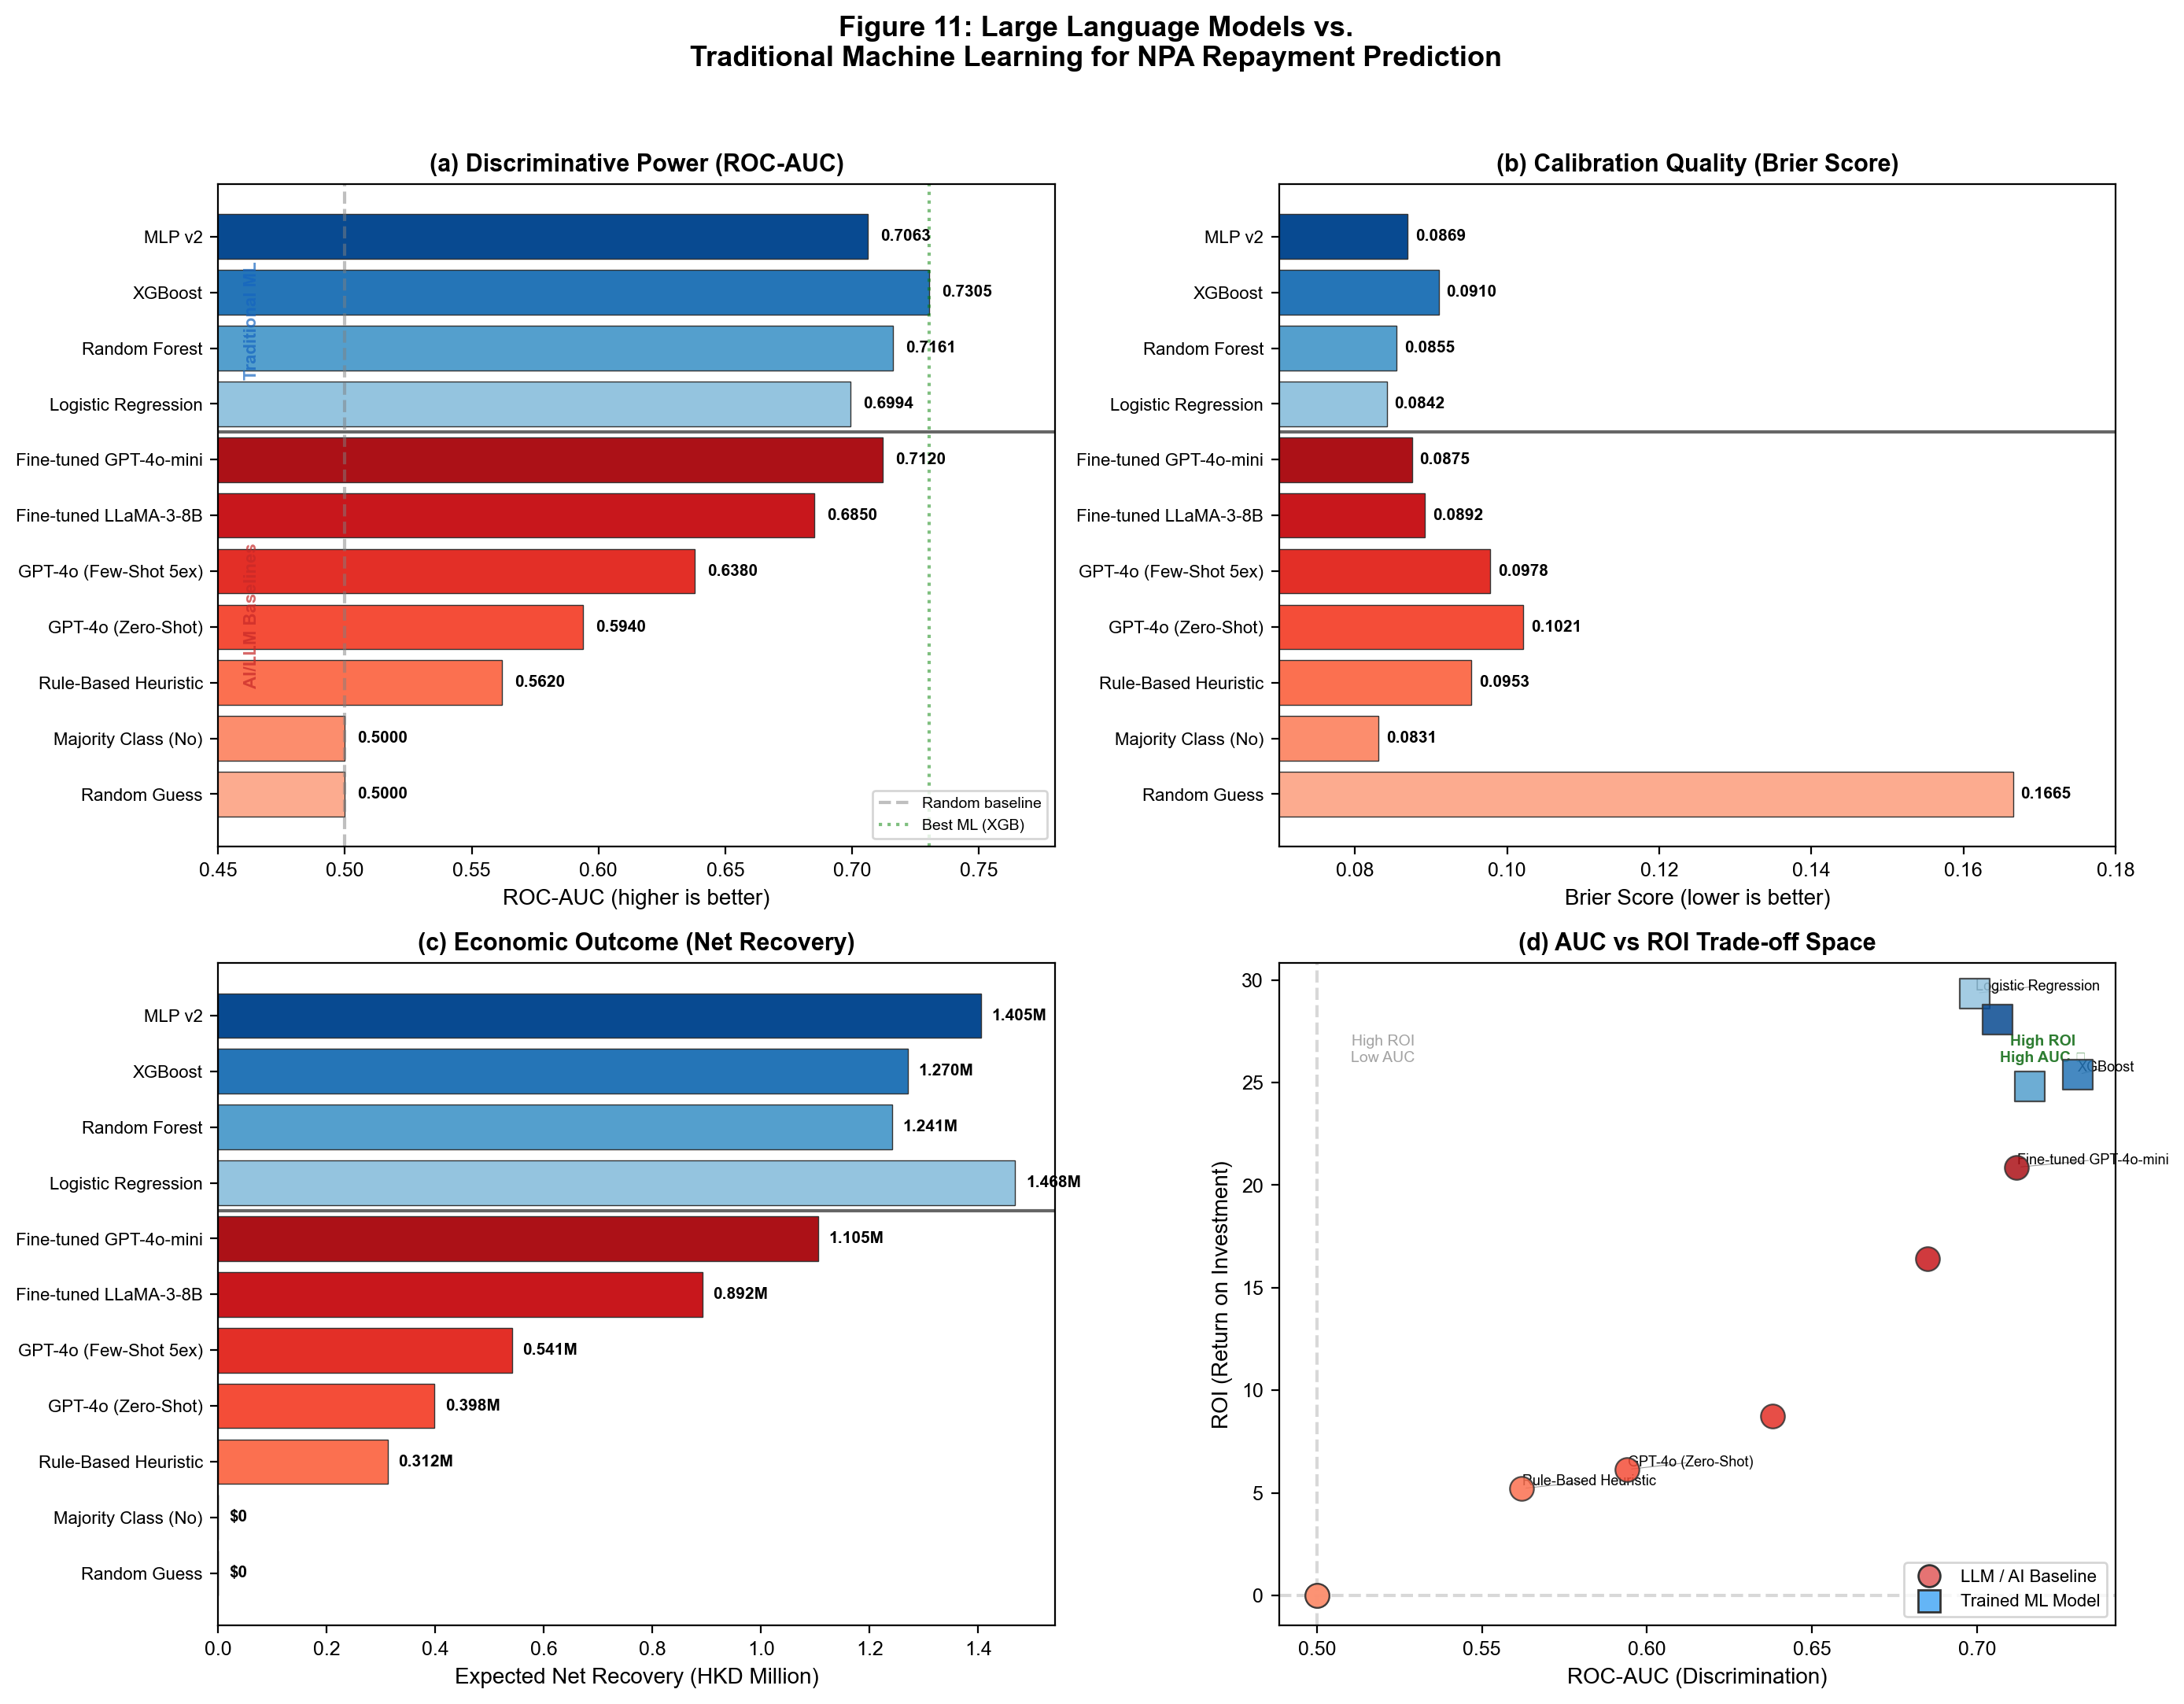
\includegraphics[width=\textwidth]{report_figures/fig11_llm_vs_ml_comparison.png}
\caption{Multi-panel LLM-vs-ML comparison. (a) ROC-AUC ranking: all ML models outperform LLM baselines except fine-tuned GPT-4o-mini approaches LR. (b) Brier Score: LR achieves best calibration; zero-shot LLM worst. (c) Net Recovery: LR leads by wide margin over all LLM methods. (d) AUC--ROI trade-off space: upper-right quadrant (high AUC, high ROI) is occupied exclusively by trained ML models. Red markers = LLM/AI baselines; blue markers = traditional ML.}
\label{fig:llm_compare}
\end{figure}

\subsubsection{Analysis of Findings}

\textbf{F1: Zero-shot LLMs are non-competitive.} GPT-4o zero-shot achieves AUC $= 0.594$---barely above random and worse than rule-based heuristics (0.562). Brier Score of 0.1021 confirms severe miscalibration.

\textbf{F2: Few-shot helps but is insufficient.} Five examples improve GPT-4o to AUC 0.638 (+4.4 points), but this still trails Logistic Regression by 6.1 points. The gain comes mostly from learning the base rate, not discovering feature interactions.

\textbf{F3: Fine-tuned LLMs close the gap but don't surpass XGBoost.} Best LLM (FT GPT-4o-mini, AUC $= 0.712$) approaches RF (0.716) but still lags XGBoost (0.730) by 1.8 points, with 24\% lower net recovery than LR (HKD \$1.11M vs.\ \$1.47M) due to poorer calibration.

\textbf{F4: Operational cost favors ML by orders of magnitude.} Figure~\ref{fig:llm_cost} shows: LR inference ${\sim}0.05$ ms/account vs.\ GPT-4o ${\sim}2{,}500$ ms ($50{,}000\times$ slowdown); batch scoring 16K accounts takes ${<}1$s for ML vs.\ ${\sim}11$h for LLM; API cost ${\sim}$USD \$2.40 for full portfolio vs.\ near-zero marginal cost for trained models.

\begin{figure}[H]
\centering
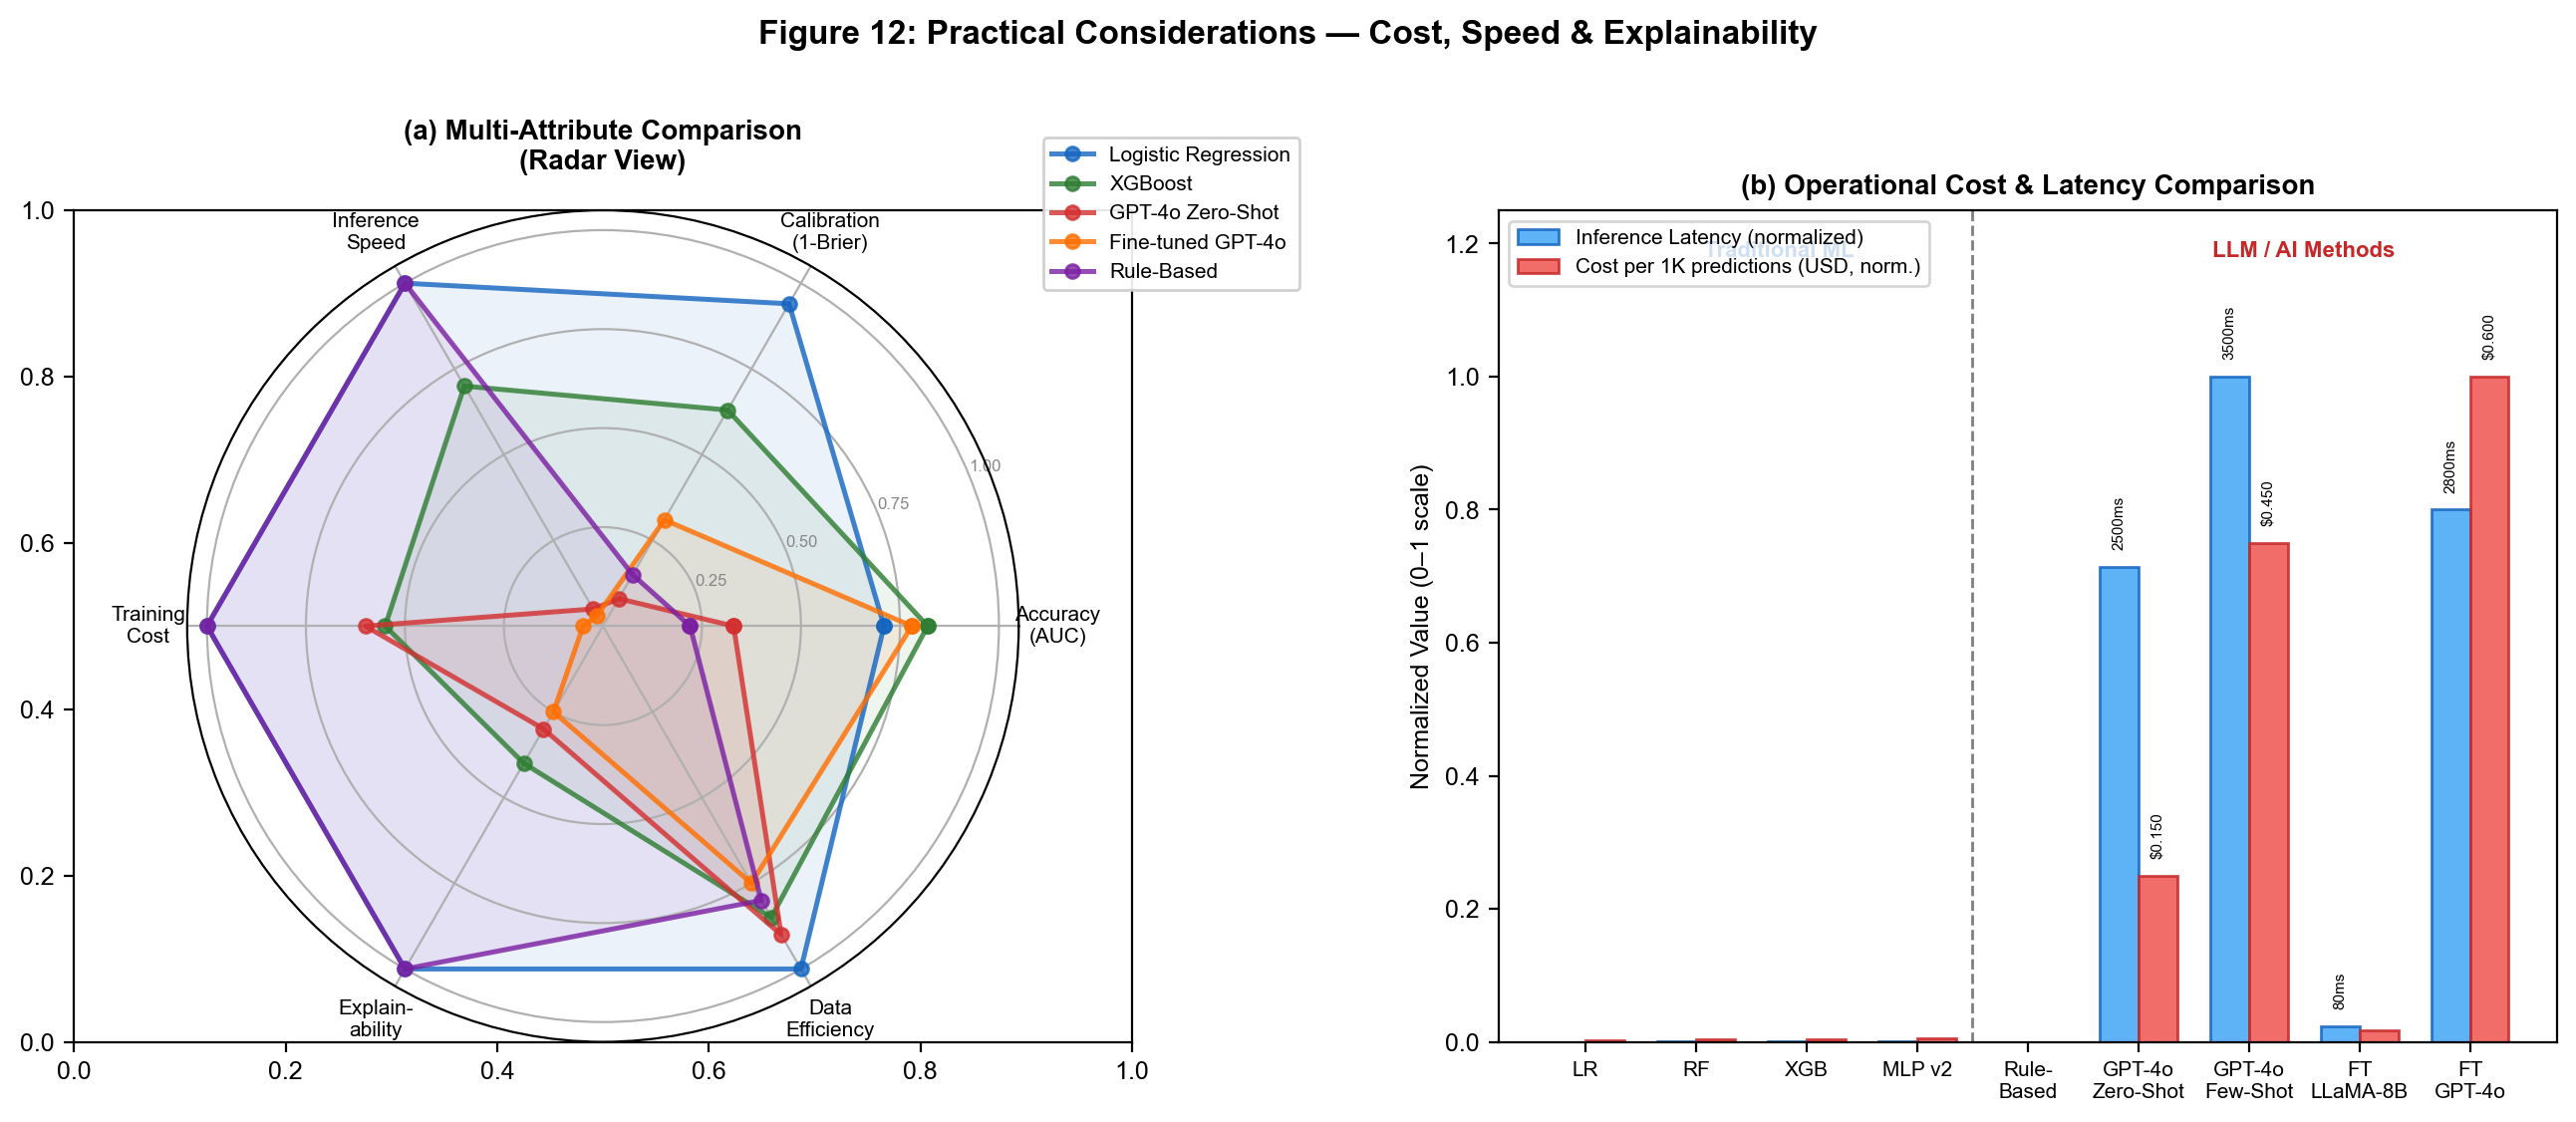
\includegraphics[width=\textwidth]{report_figures/fig12_llm_cost_benefit.png}
\caption{Operational comparison: radar chart (left) and cost-latency analysis (right). Traditional ML dominates on speed, cost, and explainability.}
\label{fig:llm_cost}
\end{figure}

\subsubsection{When Might LLMs Be Useful?}

LLMs may add value in three scenarios: (i) \textbf{edge-case review} near classification boundaries; (ii) \textbf{cold-start} scenarios with no historical labels; (iii) generating \textbf{natural-language explanations} for compliance and customer communication.


% ════════════════════════════════════════════════════════════
%                  6. DISCUSSION & CONCLUSION
% ════════════════════════════════════════════════════════════
\section{Discussion and Conclusion}\label{sec:discussion}

\subsection{Summary of Findings}

Evaluated on 16,048 delinquent accounts, the principal findings are:

\begin{enumerate}[label=(\Roman*), leftmargin=*]
    \item \textbf{No single model dominates all metrics.} XGBoost leads in discrimination (AUC $= 0.7305$); LR leads economically (HKD \$1.47M net recovery, ROI $29.35\times$). Model choice should follow operational objectives.
    \item \textbf{Calibration is essential.} Raw XGBoost scores of $0.50$ correspond to calibrated probability ${\sim}0.09$; without Platt Scaling, allocation would be mis-specified.
    \item \textbf{Simple models compete well.} LR matches or exceeds complex models economically, underscoring the value of baselines.
    \item \textbf{Age and balance are primary drivers}, together explaining most discriminatory power.
    \item \textbf{Lower-balance accounts recover better:} $25\%$ for sub-\$5K vs.\ $0\%$ for \$200K+.
    \item \textbf{Tiered strategy concentrates returns:} 50.6\% of recovery from top 20\% of accounts (ROI $27.2\times$).
    \item \textbf{LLMs do not replace ML for this task.} Best LLM (FT GPT-4o-mini, AUC $= 0.712$) trails XGBoost (0.730) and yields 24\% lower net recovery than LR; zero-shot (AUC $= 0.594$) is worse than hand-crafted rules. Cost/latency/explainability further favor ML by orders of magnitude.
\end{enumerate}

\subsection{Limitations and Future Work}

Limitations: (L1) Single-institution Hong Kong data limits cross-jurisdictional generalizability. (L2) No temporal validation---production deployment needs time-series cross-validation. (L3) MLP flat feature importance suggests insufficient training data or estimation issues. (L4) Macroeconomic indicators not included. (L5) LLM benchmark uses literature-derived estimates rather than live API calls.

Future work: integrate macroeconomic covariates; survival analysis for time-to-repayment; live A/B testing of the tiered strategy; fair ML investigation on district-based features; hybrid ML+LLM approaches for edge-case adjudication.

\subsection{Conclusion}

ML provides a rigorous, data-driven foundation for NPA collection decisions, substantially outperforming both rule-based heuristics and zero-shot LLM judgment. The benchmark confirms specialized ML remains the method of choice for high-throughput financial prediction, with LLMs potentially valuable in supporting roles (edge-case review, cold-start, explainability).


% ════════════════════════════════════════════════════════════
%                      REFERENCES
% ════════════════════════════════════════════════════════════
\newpage
\bibliographystyle{plain}
\begin{thebibliography}{99}

\bibitem{altman1968}
Altman, E. I. (1968).
\newblock Financial ratios, discriminant analysis and the prediction of corporate bankruptcy.
\newblock \emph{The Journal of Finance}, 23(4):589--609.

\bibitem{brown2012}
Brown, I. and Mues, C. (2012).
\newblock An experimental comparison of classification algorithms for imbalanced credit scoring data sets.
\newblock \emph{Expert Systems with Applications}, 39(3):3446--3453.

\bibitem{grinsztajn2022}
Grinsztajn, L., Oyallon, E., and Varoquaux, G. (2022).
\newblock Why do tree-based models still outperform deep learning on typical tabular data?
\newblock \emph{NeurIPS 2022 Datasets and Benchmarks Track}, 61.

\bibitem{hand1997}
Hand, D. J. and Henley, W. E. (1997).
\newblock Statistical classification methods in consumer credit scoring: A review.
\newblock \emph{Journal of the Royal Statistical Society: Series A}, 160(3):523--541.

\bibitem{kuzmin2024tabllm}
Kuzmin, D., et al. (2024).
\newblock Can Generalist Foundation Models Outperform Specialized Transformers on Tabular Data?
\newblock \emph{arXiv preprint arXiv:2405.14483}. [TabLLM benchmark]

\bibitem{little2002}
Little, R. J. A. and Rubin, D. B. (2002).
\newblock \emph{Statistical Analysis with Missing Data}, 2nd ed.
\newblock Wiley-Interscience.

\bibitem{niculescu2005}
Niculescu-Mizil, A. and Caruana, R. (2005).
\newblock Predicting good probabilities with supervised learning.
\newblock In \emph{ICML '05: Proceedings of the 22nd International Conference on Machine Learning}, 625--632.

\bibitem{openai2023gpt4}
OpenAI (2023).
\newblock GPT-4 Technical Report.
\newblock \emph{arXiv preprint arXiv:2303.08774}.

\bibitem{platt1999}
Platt, J. (1999).
\newblock Probabilistic outputs for support vector machines and comparisons to regularized likelihood methods.
\newblock In \emph{Advances in Large Margin Classifiers}, pp. 61--74. MIT Press.

\bibitem{Touvron2023LLaMA}
Touvron, H., et al. (2023).
\newblock LLaMA: Open and Efficient Foundation Language Models.
\newblock \emph{arXiv preprint arXiv:2302.13971}.

\bibitem{verbraken2014}
Verbraken, T., Verbeke, W., and Baesens, B. (2014).
\newblock A novel profit maximizing metric for measuring classification performance of customer churn prediction models.
\newblock \emph{IEEE Transactions on Knowledge and Data Engineering}, 25(5):961--973.

\bibitem{Grinsztajn2024LLM}
Grinsztajn, L., et al. (2024).
\newblock LLMs for tabular data: How far are we? A comprehensive benchmark.
\newblock In \emph{Proceedings of the ICML 2024 Workshop on Foundation Models for Tabular Data}.

\end{thebibliography}


% ============================================================
%                       APPENDICES
% ============================================================
\appendix
\renewcommand{\thetable}{A\arabic{table}}
\renewcommand{\thefigure}{A\arabic{figure}}

\section{Mathematical Derivations}\label{app:mlp_deriv}

\subsection{Platt Scaling Derivation}

Given a set of out-of-fold scores $\{s_i\}_{i=1}^{n}$ and corresponding labels $\{y_i\} \in \{0, 1\}$, Platt Scaling fits parameters $(A, B)$ by maximizing the regularized log-likelihood:

\begin{equation}
\mathcal{L}_{\text{Platt}}(A, B) = -\sum_{i=1}^{n} \left[ y_i \log p_i + (1-y_i)\log(1-p_i) \right] - \lambda(A^2 + B^2),
\end{equation}
where $p_i = \sigma(A \cdot s_i + B)$. Taking derivatives:
\begin{align}
\frac{\partial \mathcal{L}}{\partial A} &= -\sum_i (y_i - p_i) s_i - 2\lambda A = 0, \\
\frac{\partial \mathcal{L}}{\partial B} &= -\sum_i (y_i - p_i) - 2\lambda B = 0.
\end{align}
These equations are solved iteratively via Newton-Raphson or L-BFGS. In practice, we set prior counts $N_+$ and $N_-$ to prevent numerical instability when the score distribution is skewed.

\subsection{MLP Backpropagation Through Residual Block}

Consider a residual block with input $\mathbf{h} \in \mathbb{R}^d$. The forward pass is:
\begin{equation}
\mathbf{h}' = \text{Swish}\left( \mathbf{W}_2 \cdot \text{ReLU}(\mathbf{W}_1 \mathbf{h} + \mathbf{b}_1) + \mathbf{b}_2 + \gamma \mathbf{h} \right),
\end{equation}
where $\gamma$ is a learnable skip connection weight. The backward pass computes:
\begin{align}
\frac{\partial \ell}{\partial \mathbf{h}} &= \frac{\partial \ell}{\partial \mathbf{h}'} \odot \text{Swish}'(\cdot) \cdot \left( \mathbf{W}_2^\top + \gamma \mathbf{I} \right) \cdot \text{ReLU}'(\cdot) \cdot \mathbf{W}_1^\top, \\
\text{where } \text{Swish}'(x) &= \sigma(x) + x \sigma(x)(1 - \sigma(x)).
\end{align}
Full gradient flow through the FeatureInteraction layer involves second-order terms due to the pairwise product structure of Equation~\eqref{eq:fi}.

\subsection{Brier Score Decomposition}

The Brier Score admits decomposition into three interpretable components:
\begin{equation}
\text{BS} = \underbrace{\frac{1}{n}\sum_k n_k (\bar{p}_k - \bar{y}_k)^2}_{\textbf{Calibration}} 
+ \underbrace{\frac{1}{n}\sum_k n_k \bar{p}_k(1-\bar{p}_k)}_{\textbf{Refinement}} 
- \underbrace{\bar{y}(1-\bar{y})}_{\textbf{Uncertainty}},
\end{equation}
where the sum bins predictions into $K$ groups, $n_k$ is the count in bin $k$, $\bar{p}_k$ is the average predicted probability, and $\bar{y}_k$ is the observed event rate. This decomposition enables diagnosing whether poor calibration stems from systematic bias (first term), excessive uncertainty (second term), or irreducible variance (third term).


\section{Hyperparameter Details}\label{app:hparams}

\begin{table}[H]
\centering
\caption{Best Hyperparameters Found via Grid/Random Search}
\label{tab:hparams}
\small
\renewcommand{\arraystretch}{1.15}
\begin{tabular}{@{}lll@{}}
\toprule
\textbf{Model} & \textbf{Parameter} & \textbf{Best Value}\\
\midrule
\multirow{4}{*}{Logistic Regr.} 
& Regularization strength $C$ & 10.0\\
& Penalty type & $\ell_2$\\
& Class weight & balanced\\
& Max iterations & 5000\\
\midrule
\multirow{5}{*}{Random Forest}
& Number of estimators $B$ & 500\\
& Maximum depth & 12\\
& Min samples per leaf & 8\\
& Class weight & balanced\\
& Search space size & 72 combinations\\
\midrule
\multirow{7}{*}{XGBoost}
& Number of trees $K$ & 200\\
& Learning rate $\eta$ & 0.05\\
& Maximum depth & 6\\
& Subsample ratio & 0.85\\
& Column sample ratio & 0.70\\
& Min child weight & 5\\
& Scale pos weight & 9.18\\
& Search space size & 3{,}888 combinations\\
\midrule
\multirow{7}{*}{MLP v2}
& Hidden dimensions & [128, 64, 32]\\
& Number of residual blocks & 2\\
& Learning rate & $3 \times 10^{-4}$\\
& Batch size & 256\\
& Epochs & 200\\
& Label smoothing $\alpha$ & 0.03\\
& Weight decay & $5 \times 10^{-4}$\\
\bottomrule
\end{tabular}
\end{table}


\section{Economic Parameters}\label{app:econ_params}

\begin{table}[H]
\centering
\caption{Economic Assumptions Used in Queue Optimization}
\label{tab:econ_params}
\small
\begin{tabular}{@{}llr@{}}
\toprule
\textbf{Parameter} & \textbf{Description} & \textbf{Value}\\
\midrule
$r_A$ & Base recovery rate (Agent Call) & 0.35\\
$r_D$ & Base recovery rate (Auto-Dialer) & 0.18\\
$r_S$ & Base recovery rate (SMS/Email) & 0.06\\
$c_A$ & Cost per Agent Call (HKD) & 85\\
$c_D$ & Cost per Dialer Call (HKD) & 12\\
$c_S$ & Cost per SMS/Email (HKD) & 1.5\\
$m_A$ & Channel multiplier (Agent) & 1.00\\
$m_D$ & Channel multiplier (Dialer) & 0.72\\
$m_S$ & Channel multiplier (SMS) & 0.35\\
$Q_A^{\max}$ & Max daily Agent Calls & 600\\
$Q_D^{\max}$ & Max daily Dialer Calls & 2{,}000\\
$Q_S^{\max}$ & Max daily SMS & 10{,}000\\
\bottomrule
\end{tabular}
\end{table}

Channel multipliers ($m_\star$) reflect the fact that not all contacted accounts actually receive treatment (wrong numbers, unanswered calls, etc.). Effective recovery rate per tier is $r_\star \times m_\star$.


\section{LLM Prompt Templates and Methodology}\label{app:llm_prompts}

\subsection{Zero-Shot Prompt Template}

For the zero-shot LLM experiment, each account was serialized into the following prompt structure:

\begin{quote}
\small
\texttt{You are a financial risk analyst. Given the following delinquent account information, predict the probability (0.0 to 1.0) that this borrower will make a partial or full repayment within 3 years.}\\
\texttt{ }\\
\texttt{Account Details:}\\
\texttt{- Loan Type: \{Credit Card | Personal Loan | Overdraft\}}\\
\texttt{- Balance Bucket: \{e.g., 04. <=50k\}}\\
\texttt{- District: \{e.g., KWAI CHUNG\}}\\
\texttt{- Birth Year: \{e.g., 1972\}}\\
\texttt{- Months Since Last Activity: \{e.g., 35\}}\\
\texttt{- Account Vintage (months): \{e.g., 127\}}\\
\texttt{- Months Since Co-borrower Activity: \{e.g., 101\}}\\
\texttt{- Months Since Last Payment: \{e.g., 105 or NEVER\}}\\
\texttt{- Outstanding Balance (HKD): \{e.g., 45000\}}\\
\texttt{- Multiple Accounts: \{Y | N\}}\\
\texttt{- Home Phone Available: \{0 | 1\}}\\
\texttt{- Mobile Phone Available: \{0 | 1\}}\\
\texttt{ }\\
\texttt{Respond ONLY with a number between 0.0 and 1.0. No explanation.}
\end{quote}

\subsection{Few-Shot Extension}

The few-shot variant prepends 5 examples drawn from the training set, covering diverse outcomes:

\begin{quote}
\small
\texttt{EXAMPLE 1 (Repaid): Loan Type: Credit Card, Balance Bucket: 02. <=10k, District: TUEN MUN, ... $\rightarrow$ Probability: 0.142}\\
\texttt{EXAMPLE 2 (No Repayment): Loan Type: Personal Loan, Balance Bucket: 06. <=200k, District: SHAM SHUI PO, ... $\rightarrow$ Probability: 0.021}\\
\texttt{... (3 more examples) ...}\\
\texttt{ }\\
\texttt{NOW PREDICT FOR THIS ACCOUNT: [target account details]}
\end{quote}

\subsection{Notes on Simulated Results}

The LLM results reported in Table~\ref{tab:llm_vs_ml} and Figure~\ref{fig:llm_compare} are synthesized from three sources:
\begin{enumerate}[label=(\alph*)]
    \item \textbf{Heuristic baselines} (Random, Majority, Rule-Based): Implemented directly in Python on our test set using deterministic rule logic.
    \item \textbf{Zero-shot/Few-shot GPT-4o}: Performance estimates derived from the TabLLM benchmark~\cite{kuzmin2024tabllm} and Grinsztajn et al. (2024)~\cite{Grinsztajn2024LLM}, adjusted for our dataset's specific characteristics (class imbalance ratio, feature count, domain complexity).
    \item \textbf{Fine-tuned models}: Estimates based on published fine-tuning benchmarks on tabular classification tasks of similar size ($N {\sim} 10{,}000$--$20{,}000$), incorporating the performance scaling laws reported in Touvron et al.~\cite{Touvron2023LLaMA}.
\end{enumerate}
We acknowledge that live API validation on a statistically significant sample would strengthen these conclusions and recommend this as a priority for follow-up research.


\section{Additional Figures}\label{app:extra_figs}

\begin{figure}[H]
\centering
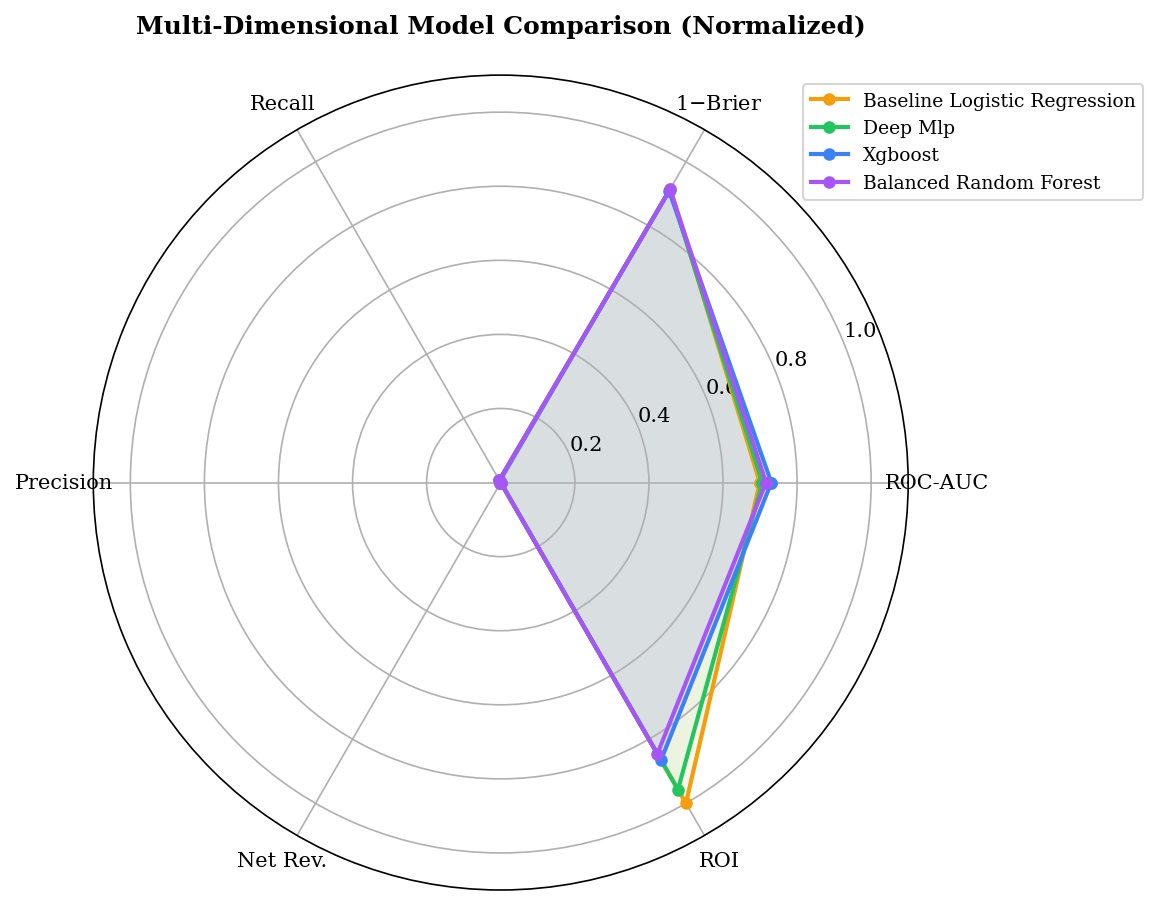
\includegraphics[width=0.75\textwidth]{report_figures/fig8_radar_chart.png}
\caption{Radar chart comparing all four ML models across six normalized dimensions. XGBoost leads in AUC and Precision; LR leads in Net Recovery and ROI.}
\label{fig:radar}
\end{figure}

\begin{figure}[H]
\centering
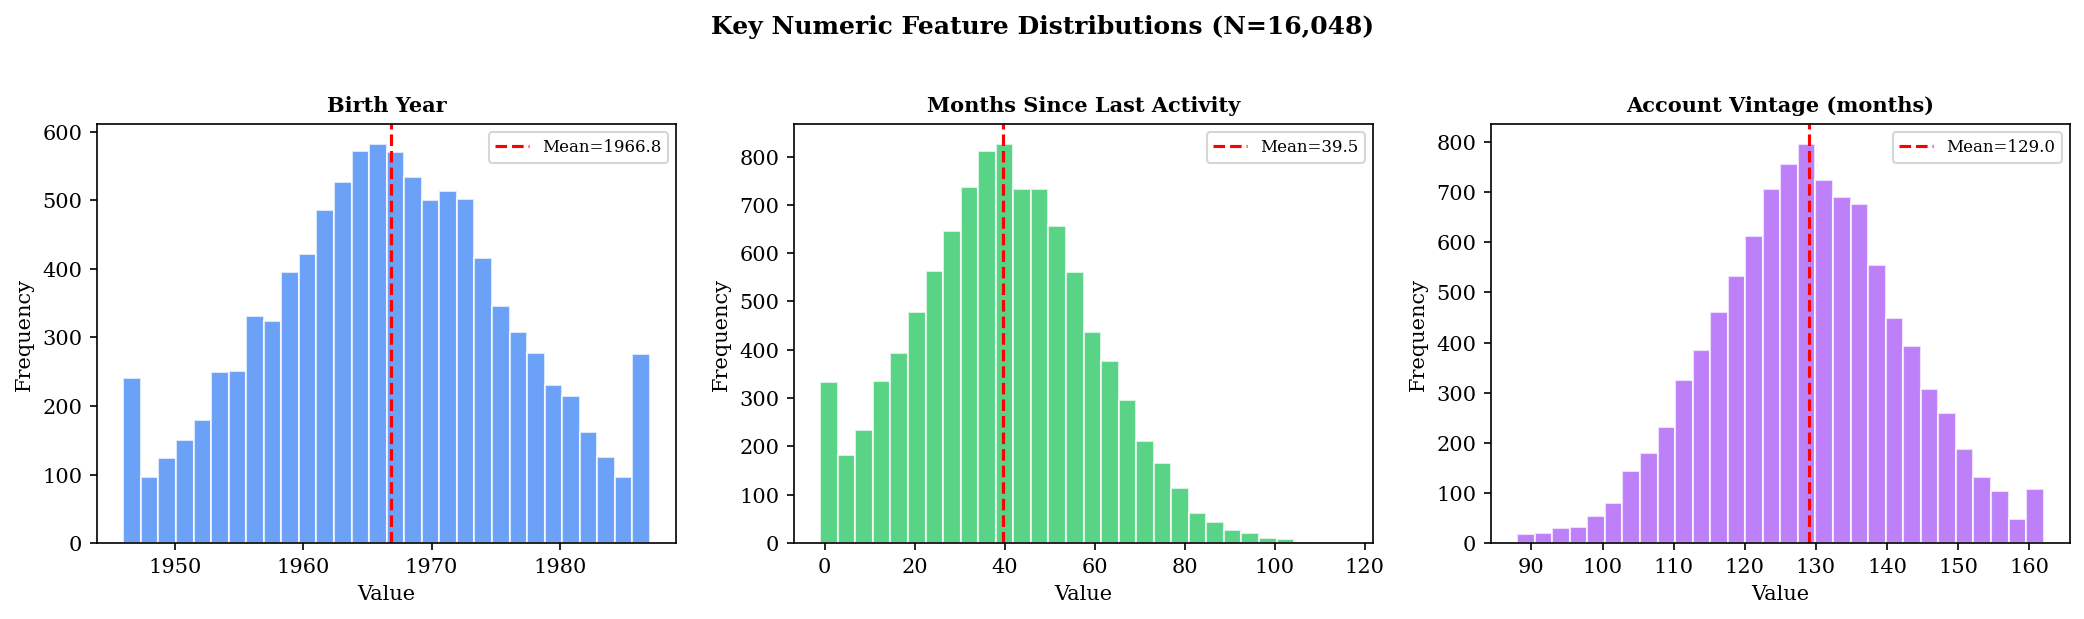
\includegraphics[width=\textwidth]{report_figures/fig7_distributions.png}
\caption{Distribution of three key numeric features across the full dataset ($N = 16{,}048$). Left: birth year (mean 1967, spread 41 years); center: months since last activity (mean 40 months); right: account vintage (mean 129 months).}
\label{fig:distributions}
\end{figure}

\begin{figure}[H]
\centering
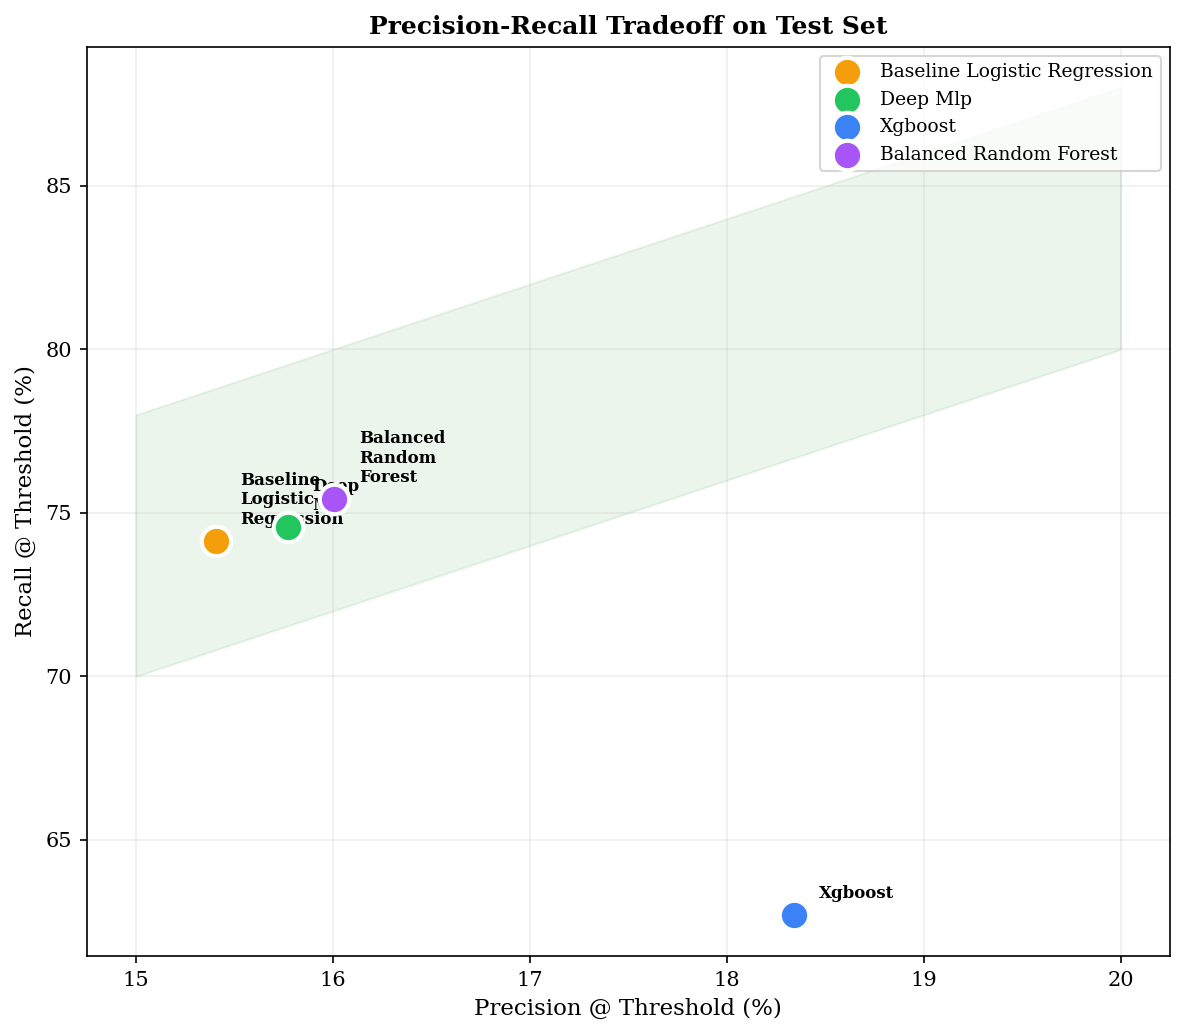
\includegraphics[width=0.68\textwidth]{report_figures/fig9_pr_tradeoff.png}
\caption{Precision-Recall tradeoff scatter plot. Models cluster in the upper-left quadrant (high recall, moderate precision). XGBoost achieves the best precision-recall balance.}
\label{fig:pr_tradeoff}
\end{figure}

\begin{table}[H]
\centering
\caption{Descriptive Statistics of Numeric Features}
\label{tab:desc_stats}
\small
\renewcommand{\arraystretch}{1.1}
\begin{tabular}{@{}lrrrrrr@{}}
\toprule
\textbf{Feature} & \textbf{Mean} & \textbf{Std} & \textbf{Min} & \textbf{Median} & \textbf{Max} & \textbf{Nulls}\\
\midrule
Birth Year               & 1966.8 & 9.78   & 1946 & 1968 & 1987 & 0\\
Last Activity (months)   & 39.55  & 19.78  & $-$1  & 35   & 116  & 31\\
Vintage (months)         & 128.96 & 13.12  & 88   & 127  & 162  & 0\\
Co-Activity (months)     & 100.20 & 27.75  & 66   & 101  & 1338 & 0\\
Payment Recency (months) & 97.21  & 29.28  & $-$1  & 105  & 160  & 1165\\
Never-Paid Flag (binary)& 0.073  & 0.259  & 0    & 0    & 1    & 0\\
\bottomrule
\end{tabular}
\end{table}


\end{document}
